\setchapterimage[7cm]{nuclear/nuclear_sample_cutouts.png}
\chapter{The Nuclear Sample}\label{nucsam}
\labch{nuclear}
Motivated\marginnote{Cutouts of several transients in the nuclear sample, as seen in the ZTF \textit{g}-band near optical peak.} by the three neutrinos coincident with accretion phenomena in the cores of active galaxies, I created a systematic sample of nuclear transients in the ZTF footprint. No such sample existed, as AGN studies are usually interested in long-term variability of galaxies, while transient studies are normally excluding phenomena too close to galaxy cores as contaminants. Such a systematic sample of partially unclassified transient phenomena might provide additional insights into the physics of galactic nuclei.

Furthermore, with the advent of a deep high-cadence sky surveys in the form of the Legacy Survey of Space and Time (LSST, hosted by the Vera C. Rubin Observatory)~\sidecite{Ivezic2019} in the near future, photometric identification of transients will be crucial.

The rate of transients detected by LSST will by far exhaust the available spectroscopic resources, thus requiring informed decisions about when to rely on spectroscopy for classification and characterization. The vast majority of LSST-detected transients will either be photometrically classified, or not classified at all. Therefore, photometrically classifying the ZTF nuclear transients can serve as a precursor study to LSST-era astronomy.

This chapter is dedicated to transients \textbf{similar to the three transients for which a neutrino association could be made}: Nuclear transients, i.e.~transients observed \textbf{close to the cores of their galaxies}. Because no clear picture on the composition of such a sample exists, we gathered one and made a first attempt at classifying it.

The routines used to create and classify the nuclear sample were written in Python, and are accessible online\sidenote{\url{https://github.com/simeonreusch/ztfnuclear}}.

\section{Sample Creation}
The nuclear sample was created with \texttt{AMPEL} (see Section~\ref{ampel}), using its capability to rerun analyses on archival data. To perform such a rerun, a modified version of the \texttt{AMPEL} nuclear filter was used\sidenote{\url{https://github.com/AmpelAstro/Ampel-nuclear}}.

\subsection{\texttt{AMPEL} Nuclear Filter}\label{nuclear_filter}

This filter is used primarily by the ZTF TDE working group to scan for transient activity that is compatible with an emerging TDE~\cite{Velzen2021a}. In the rerun, it was slightly modified, and used to evaluate each and every alert issued by ZTF.

The logic behind the filtering process can be explained as follows: It selects events with a minimum of photometric quality, ensured by minimum requirements on the number of detections and the brightness. The event at least once needs to pass as `real' (opposed to bogus), and the host needs a high probability of passing as galaxy, not star. Furthermore, \textit{Gaia} is consulted to veto against stars, and the events need to be nuclear, i.e.~happen close to the core of their host galaxy.

\begin{marginfigure}
  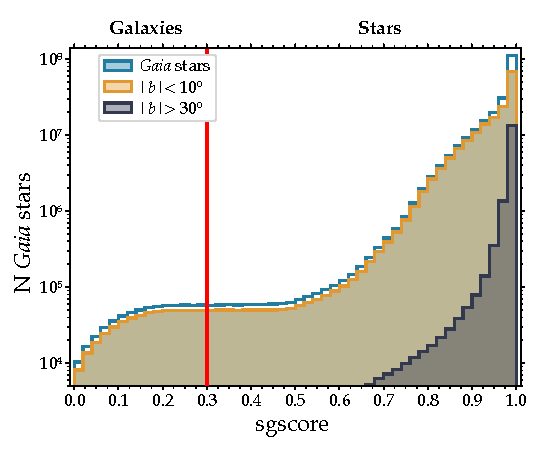
\includegraphics{nuclear/sgscore.pdf}
  \caption[\texttt{sgscore} performance]{\texttt{sgscore} performance evaluated with known \textit{Gaia} stars. At the chosen threshold of 0.3 (red line), the misidentification of stars as galaxies is negligible. Adapted from~\cite{Tachibana2018}}
  \labfig{sgscore}
\end{marginfigure}

The criteria used were:
\begin{description}
  \item[\texttt{sgscore}] As detailed in Section~\ref{ztf_image_subtraction}, \texttt{sgscore} is a machine-learning based star-galaxy score for PS1 objects (low values: galaxy, high values: stars). The transient must at least once have an \texttt{sgsscore} < 0.3 to pass the filter.
  \item[Number of detections] At least 3 detections in both ZTF \textit{g}- and \textit{r}-band are required.
  \item[Galactic cut] The object must be separated by at least \SI{5}{\degree} from the galactic plane to avoid contamination by foreground stars.
  \item[PS1 photometry] To avoid crowded areas, transients where more than 100 objects in the vicinity have a counterpart in PS1 are removed.
  \item[Brightness] At least one alert datapoint of the transient must be brighter than 20 mag.
  \item[\texttt{rbscore}] The real-bogus score separating erroneous detections (low values) from real ones (high values, see Section~\ref{ztf_alerts}) must be larger than 0.3. Note that for more recent data, also \texttt{deep real bogus} is available, which promises vastly better results~\sidecite{Duev2019}. Older alerts from 2018 or 2019 do not contain this information, and there is no direct translation from an \texttt{rbscore} threshold to a \texttt{drbscore} threshold. For these reasons and to maximize consistency, we restricted ourselves to using only the older \texttt{rbscore}. The quite loose cut of 0.3 does not entail overly large contamination, as we also required the transient to have a PS1 counterpart. Figure~\ref{fig:rbvsdrb} shows a comparison of the False Negative Rate (FNR) of \texttt{rbscore} vs. \texttt{drbscore}. At the chosen threshold of $0.3$, the FNR for both algorithms is a the percent level.
  \item[Core distance] For all objects that made it this far, their angular distance to the core was computed. To make this more robust, three different distance metrics were computed. The \textbf{mean distance} to the PS1 source in the reference images, the \textbf{median distance} to that, and lastly, a \textbf{weighted distance}. The latter was computed according to~\sidecite{Velzen2019} and accounts for the fact that the RMS of the angular core distance scales linearly with magnitude. $\sigma_\text{dist}$ = $0.24 + 0.04(m-20)$, where $m$ is the difference photometry magnitude. This stage accepts all transients for which at least one of the three angular distances lies below 0.5 arcseconds.
\end{description}

\begin{figure}[htpb]
  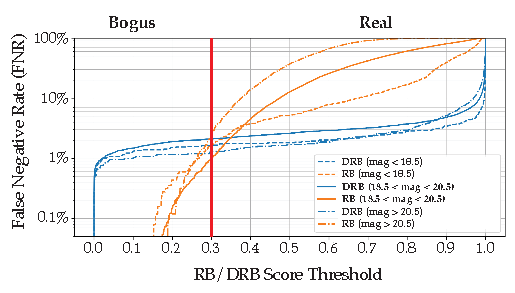
\includegraphics[width=0.9\textwidth]{nuclear/rb_v_drb.pdf}
  \caption[\texttt{rbscore}/\texttt{drbscore} performance]{\texttt{rbscore} vs \texttt{drbscore} performance, evaluated in terms of false negative rate as a function of the threshold. Adapted from~\cite{Duev2019}. The chosen threshold of 0.3 is shown as red vertical line. At that value, \texttt{rbscore} has a False Negative Rate of \SI{\approx1}{\percent} in the relevant magnitude range of $18.5 < \text{mag} < 20.5$.}
  \labfig{rbvsdrb}
\end{figure}

This filter was then applied to all ZTF alerts issued between 1 April, 2018 and 30 April, 2022, comprising over 4 years of data in total.

\subsection{Rejection Statistics}
From a total sample of $\sim 350$ Million alerts issued by ZTF during these 4 years, ultimately 11687 nuclear transients were selected. The survival rates during the filtering process are shown in Fig.~\ref{fig:nuclear_decision}, with complete alert stream on top, different thematically grouped rejection stages in between and the final accepted alerts on the bottom. In total, \SI{0.2}{\percent} of alerts issued by ZTF were accepted by the filter.

\begin{figure}[h!]
  \begin{tikzpicture}[node distance=1.4cm]
    \node (start) [keep] {355,429,833 initial ZTF alerts};
    \node (dec1) [decision,  font=\small, align=center, below of=start] {SQL Filter};
    \node (expl1) [explain, font=\small, align=left, left of=dec1, xshift=-1.8cm] {$<20$ mag\\\texttt{rbscore} $>0.3$\\PS1 dist $<0.5$ arcsec\\$\geq 3$ detections};
    \node (disc1) [discard, font=\small, right of=dec1, xshift=2.48cm] {Discard alerts};
    \node (dec1a) [decision, font=\small, align=center, below of=dec1] {Transient\\already accepted?};
    \node (keep1) [keep, font=\small, below of=dec1a] {Keep 81,387,053 alerts};
    \node (dec2) [decision, font=\small, align=center, below of=keep1] {\texttt{sgscore}\\veto};
    \node (expl2) [explain, font=\small, align=left, left of=dec2, xshift=-2.2cm] {\texttt{sgscore} $\leq0.3$};
    \node (disc2) [discard, font=\small, right of=dec2, xshift=2.44cm,align=center] {Discard\\81,204,804\\alerts};
    \node (keep2) [keep, font=\small, below of=dec2] {Keep 182,080 alerts};
    \node (dec3) [decision, font=\small, align=center, below of=keep2] {PS1\\veto};
    \node (expl3) [explain, font=\small, align=left, left of=dec3, xshift=-1.5cm] {PS1 source faint enough\\good PS1 photometry};
    \node (disc3) [discard, font=\small, right of=dec3, xshift=2.5cm, align=center] {Discard\\20,331 alerts};
    \node (keep3) [keep, font=\small, below of=dec3] {Keep 161,749 alerts};
    \node (dec4) [decision, font=\small, align=center, below of=keep3] {Photometry\\veto};
    \node (expl4) [explain, font=\small, align=left, left of=dec4, xshift=-1.5cm] {$<20$ mag\\$\geq$ 3 detections\\flux increase $>2.5$ mag};
    \node (disc4) [discard, font=\small, right of=dec4, xshift=2.5cm, align=center] {Discard\\68,985 alerts};
    \node (keep4) [keep, font=\small, below of=dec4] {Keep 92,764 alerts};
    \node (dec5) [decision, font=\small, align=center, below of=keep4] {Position\\veto};
    \node (expl5) [explain, font=\small, align=left, left of=dec5, xshift=-1.5cm] {$>5$ deg from gal. plane\\not potential mover};
    \node (disc5) [discard, font=\small, right of=dec5, xshift=2.5cm, align=center] {Discard\\38,600 alerts};
    \node (keep5) [keep, font=\small, below of=dec5] {Keep 54,164 alerts};
    \node (dec6) [decision, font=\small, align=center, below of=keep5] {\textit{Gaia}\\veto};
    \node (expl6) [explain, font=\small, align=left, left of=dec6, xshift=-1.5cm] {No match to \textit{Gaia} star\\$\leq30$ \textit{Gaia} stars close by};
    \node (disc6) [discard, font=\small, right of=dec6, xshift=2.5cm, align=center] {Discard\\42,477 alerts};
    \node (keep6) [keep, font=\small, below of=dec6] {Keep 723,053 alerts};
    \node (keep7) [keepfinal, font=\small, below of=keep6] {Keep 11,687 transients};
    \draw [arrow] (start) -- (dec1);
    \draw [arrow] (keep1) -- (dec2);
    \draw [arrow] (dec1) -- node[midway,above] {\small no} (disc1);
    \draw [arrow] (dec1) -- node[midway,left] {\small yes} (dec1a);
    \draw [arrow] (dec2) -- node[midway,above] {\small no} (disc2);
    \draw [arrow] (dec2) -- node[midway,left] {\small yes} (keep2);
    \draw [arrow] (dec1a) -- node[midway,left] {\small no} (keep1);
    \draw [arrow] (keep2) -- (dec3);
    \draw [arrow] (dec3) -- node[midway,above] {\small no} (disc3);
    \draw [arrow] (dec3) -- node[midway,left] {\small yes} (keep3);
    \draw [arrow] (keep3) -- (dec4);
    \draw [arrow] (dec4) -- node[midway,above] {\small no} (disc4);
    \draw [arrow] (dec4) -- node[midway,left] {\small yes} (keep4);
    \draw [arrow] (keep4) -- (dec5);
    \draw [arrow] (dec5) -- node[midway,above] {\small no} (disc5);
    \draw [arrow] (dec5) -- node[midway,left] {\small yes} (keep5);
    \draw [arrow] (keep5) -- (dec6);
    \draw [arrow] (dec6) -- node[midway,above] {\small no} (disc6);
    \draw [arrow] (dec6) -- node[left] {\small yes} (keep6);
    \draw [arrow] (dec1a.east) -- ++(4,0) node[midway,above]{\small yes} |- (keep6.east);
    \draw [arrow] (keep6) -- node[midway,left] {\small translates to} (keep7);
  \end{tikzpicture}
  \caption[Nuclear filter flow chart]{Flow chart showing the rejection statistics of the nuclear filter.}
  \labfig{nuclear_decision}
\end{figure}

As one can see, the vast majority of alerts were rejected based on them being either too faint, likely being bogus, or likely being stars. The majority of alerts already get filtered by the initial SQL query. The SQL-based filtering was also the most efficient one, so the author made sure that the amount of filtering at that stage (on the archive server) was maximized.

This was followed by the live transfer all surviving alerts to another machine and processing of the subsequent filtering stages. In total, the filtering process took roughly 5 weeks.

\subsection{Forced photometry}
To be sensitive to early and late-time light curve evolution, forced photometry was acquired for all 11687 transients making the final cut. This was again done with \texttt{fpbot}, see Section~\ref{fpbot} for details. The process proved cumbersome due to the enormous data volume (several hunders of GB) that was required to be transferred from IPAC and stored in batches due to computing center restrictions.

\subsection{Infrared Data}\label{irdata}
Motivated by the strong dust echo detected for \textit{AT2019dsg}, \textit{AT2019fdr} and \textit{AT2019aalc}, the optical forced photometry dataset was completed with infrared light curves from the \textit{WISE} mission. These were obtained to serve in a selection of interesting transients based on their infrared dust echo, see Section~\ref{dustecho_sel}.

Data retrieval was performed with the \texttt{timewise} package~\sidecite{Necker2023a} to download all datapoints available for each source location in the \textit{W1}- and \textit{W2}-band. The tool automatically crossmatched the ZTF transient position to the \textit{WISE} light curve repository, downloaded the raw photometry for each source and binned the single source exposures of each epoch, spaced in half-year intervals.

\textbf{Most sources did have infrared counterparts}. To obtain a selection of likely \textbf{dust-echo candidates}, an \texttt{AMPEL} package was used, namely \texttt{T2DustEchoEval}, to analyze the infrared light curves with a Bayesian block algorithm in order to identify periods of flaring activity compared to a baseline; see also Section~\ref{bayesian_blocks} for a discussion of the same algorithm utilized for ZTF optical data.

The significance of these flares was then calculated with a metric dubbed \textbf{dust echo strength}. This was defined in~\cite{Velzen2021} as $\Delta F_\text{IR}/F_\text{RMS}$, where $\Delta F_\text{IR}$ is the difference between the flaring period flux and the baseline flux; $F_\text{RMS}$ is the root-mean square of the baseline flux.

\subsection{Catalog Matching}
To enrich the sample by information available on the transients, these were crossmatched to a variety of catalogs and services. The results of the crossmatches were stored locally in a \texttt{MongoDB} database for ease of retrieval. The crossmatches were either used to extract training features (e.g.~\textit{textit{WISE}} colors) or evaluate the quality of the trained models (e.g.~Marshal/Fritz or TNS). In detail, these crossmatches comprised:

\begin{description}
  \item[Spectroscopic Redshifts] To obtain \textbf{spectroscopic redshifts}, the \texttt{AMPEL} module \texttt{T2DigestRedshifts} was employed. This queries the following services: A local database of the spectroscopic redshifts contained in the NASA/IPAC Extragalactic Database (NED)\sidenote{\url{https://ned.ipac.caltech.edu}}, spectroscopic redshifts from SDSS, and finally spectroscopic redshifts from the Galaxy List for the Advanced Detector Era (GLADE)~\sidecite{Dalya2018} v2.3.
  \item[Photometric Redshifts] Additionally, \texttt{T2DigestRedshifts} also provided \textbf{photometric redshifts} from the Legacy Survey~\sidecite{Zhou2020}, the 2MASS Photometric Redshift Catalog~\sidecite{Bilicki2013}, and photometric redshifts from the PS1 Source Types and Redshifts with Machine learning (PS1-STRM) catalog~\sidecite{Beck2020} as well as GLADE.
  \item[Marshal/Fritz] During ZTF Phase I, the GROWTH Marshal~\sidecite{Kasliwal2019} served as a community hub to gather information on single transients. It provided a web interface to upload spectroscopy, discuss photometry and add classifications and redshift. This service has been replaced by Fritz~\sidecite{Coughlin2023} with the same design goal, but greater modularity and API support. Both services were queried for transient classifications and redshifts.
  \item[TNS] The Transient Name Server (see Section~\ref{catmatch}) was also used to obtain classifications and redshifts of known transients.
  \item[AllWISE] Additionally to the \textit{WISE} light curves, archival data from the first part of the \textit{WISE} mission was obtained. This had the advantage of providing two additional bands reaching into the far infrared (\textit{W3} and \textit{W4}), which were deactivated after the nominal mission end of \textit{WISE} due to lack of coolant. These allowed for the calculation of more colors. This was used in AGN rejection, see Section~\ref{agn_rejection}.
  \item[CRTS DR1] The Catalina Real-time Transient Survey Catalog contains cataclysmic variables which were crossmatched against to reduce contamination by foreground stars.
  \item[SDSS] The Sloan Digital Sky Survey was also used to crossmatch against foreground stars.
\end{description}

\section{Creating Features: Light Curve Fits}
To photometrically classify the transients, the following strategy was employed: \textbf{Fit all transients} with a dedicated \textbf{TDE light curve model}, as well as a \textbf{supernova Ia model}. These features, appended by \textbf{additional features}, can serve as a base to classify the nuclear sample. Such a training task requires a truth on which to train on. The truth base chosen here was the BTS sample, which was augmented by creating copies of existing objects, as well as adding new, underrepresented transients. All those steps will be explained below.

\subsection{Fitting a TDE Model}\label{tde_model}
To model a TDE-like source evolution, a variation of the parametrization presented in~\cite{Velzen2021a} was used.

\subsubsection{TDE Parametrization}
The basic  idea is to fit the light curve evolution with a Gaussian rise and exponential decay of a blackbody, which can also linearly change in temperature over a certain amount of time. The luminosity evolution is then given by

\begin{equation}
  L(t,\lambda) = \frac{T_\text{peak}^4}{T(t)^4} B_\lambda F(t),
\end{equation}
where $\lambda$ is the evaluated wavelength, $T_\text{peak}$ is the blackbody temperature at peak, $T(t)$ is its temperature at time $t$ and $B(t)_\lambda$ is the spectral radiance of the blackbody
\begin{equation}
  B(t)_\lambda = \frac{2 c h}{\lambda^5} \frac{1}{\exp(\frac{hc}{\lambda k_B T(t)})-1},
\end{equation}
and $F(t)$ is the Gaussian rise pre-peak and exponential decay post peak:
\begin{equation}
  F(t) = \begin{cases}
    \exp[-(t-t_\text{peak})^2/2\sigma^2] & \text{if } t\leq t_\text{peak} \\
    \exp[-(t-t_\text{peak})/\tau]        & \text{otherwise.}
  \end{cases}
\end{equation}
Here, $\sigma$ is the rise time of the transient, and $\tau$ is the decay time, both in days.

Lastly, $T(t)$ was allowed to change linearly during an interval after $t_\text{peak}$ until $t_\text{cutoff}$, marking the end of the linear temperature evolution:
\begin{equation}
  T(t) = \begin{cases}
    T_\text{peak}                    & \text{if $t<t_\text{peak}$}                              \\
    T_\text{peak} + t \cdot \Delta T & \text{if $~t_\text{peak} \leq t \leq t_\text{cutoff} $ } \\
    T_\text{cutoff}                  & \text{otherwise},
  \end{cases}
\end{equation}
with $\Delta T$ being the coefficient of temperature change. Also, there was a check that required at least 10 datapoints within the interval 30 days prior to peak time and one year after that. If that check did not succeed, the fit was set to fail due to poor source sampling.

As a source luminosity can only be calculated when the redshift is known, and this was not true for a majority of the nuclear transients, an arbitrary amplitude was used instead. This does not affect the results in any meaningful way, as TDEs can differ in brightness by at least two orders of magnitude (see e.g.~\cite{Hammerstein2022}), and only the shape of the light curve is relevant for the goodness of fit.\cite{Hammerstein2022}

This model has been realized as an instantiation of an \texttt{SNCosmo} source model, as this package has the advantage of built in filter profiles, that allowed the correct evaluation of the blackbody flux as seen through the ZTF filters. To save computing time, the fit algorithm used was not a Markov-Chain Monte Carlo as in~\cite{Velzen2021a}, but \texttt{iminuit/MIGRAD}.

To account for Milky Way dust extinction along the line of sight, the infrared dust maps by Schlegel, Finkbeiner y \& Davis were used~\sidecite{Schlegel1998}, as provided by the \texttt{sfdmap}\sidenote{\url{https://github.com/kbarbary/sfdmap}} Python package.

\subsubsection{TDE Fit Priors}
To constrain the fits and mitigate runaway, fit priors were used, partly taken from~\cite{Velzen2021a}. These are shown in Table~\ref{tab:tde_fit_priors}.

The prior on the time of peak, here dubbed $t_0$, was inferred from a peak finding algorithm that identified the highest flux point in each band (given it had a signal-to-noise ratio of $>3$) after smoothing the light curve with a rolling window, calculating the median flux within a widow width of 10 days.

\begin{table}[h]
  \begin{center}
    \begin{tabular}{c c c c}
      \hline
      \textbf{Param.}      & \textbf{Description} & \textbf{Prior} & \textbf{Bounds}                     \\
      \hline
      \hline
      $t_\text{peak}$      & Peak time            & $t_0$          & $t­_0 \pm 30$ days                  \\
      $\log T_\text{peak}$ & Peak temperature     & 4 K            & [3.5, 5]~\unit{\K}                  \\
      $\log \sigma$        & Gaussian rise time   & 1.6 days       & [0,5] days                          \\
      $\log \tau$          & Exp. decay time      & 2.3 days       & [0,5] days                          \\
      $\Delta T$           & Temp. change / day   & 0              & $T_\text{peak} \pm 15000$ K (total) \\
      $t_\text{cutoff}$    & End of temp. evol.   & 300            & [100, 1200] days $+t_0$             \\
      \hline
    \end{tabular}
  \end{center}
  \caption[TDE Fit priors]{Priors for the TDE fit.}\label{tab:tde_fit_priors}
\end{table}

As the blackbody fits were not constrained by UV data, in some cases \textbf{temperature runaway} occured when allowing all fit parameters to vary freely within their bounds. This can be explained as follows: A decrease in brightness over time can be either be achieved by exponential decay or by an increase in temperature. The latter gradually moves the blackbody spectrum outside the ZTF bands, which then translates to decreasing brightness. As such excessive temperature changes are most likely unphysical, the daily temperature change $\Delta T$ was limited to an integrated maximum change of $T_\text{peak} \pm \SI{1.5e4}{\K}$.

Another measure to mitigate the issue was to perform the fits as a \textbf{two-stage process}: First, the temperature evolution was disabled, i.e. $\Delta aT$ was set to $0$ and $t_\text{cutoff}$ was removed as parameter, with the blackbody only having one temperature for the duration of the light curve, $T_\text{peak}$. The best-fit values for $t_\text{peak}$, $\log T­­_\text{peak}$, $\log \sigma$ and $\log \tau$ obtained in this first stage were then used as fit priors for stage 2. This procedure solved the temperature runaway in almost all cases.

\begin{figure}[htb]
  \centering
  \begin{subfigure}[b]{0.49\textwidth}
    \centering
    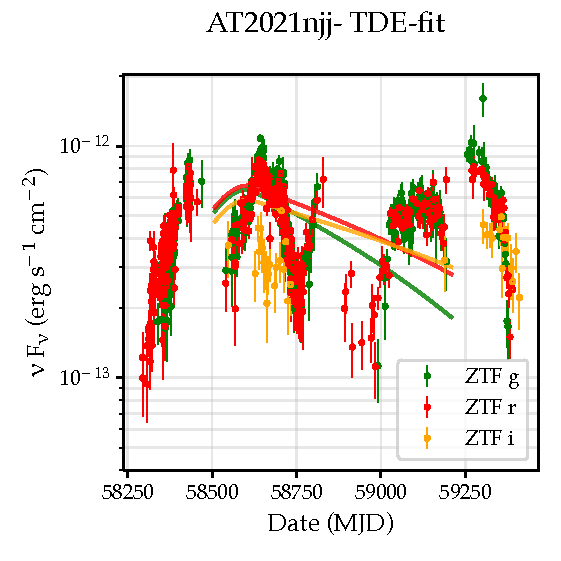
\includegraphics[width=1\textwidth]{nuclear/ZTF18aaymybb_exp.pdf}
  \end{subfigure}
  \begin{subfigure}[b]{0.49\textwidth}
    \centering
    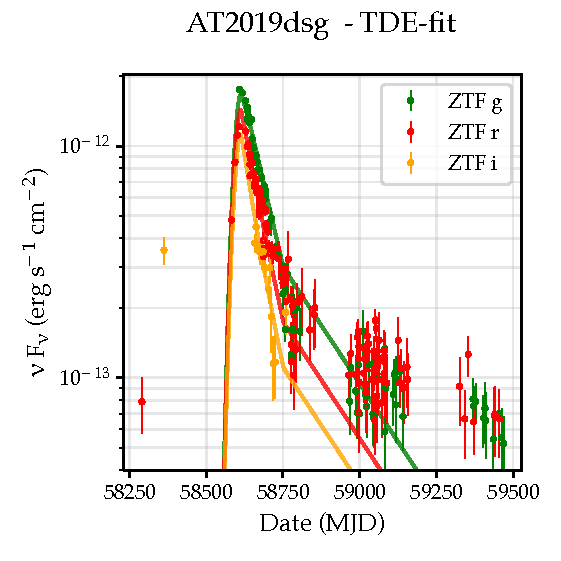
\includegraphics[width=1\textwidth]{nuclear/ZTF19aapreis_exp.pdf}
  \end{subfigure}
  \caption[Two exemplary TDE fits]{Two exemplary TDE light curve fits. \textbf{Left}: \textit{AT2021njj}, displaying periodic AGN activity not well captured by the fit.\ \textbf{Right}: \textit{AT2019dsg}, a TDE which is captured fairly well by the fit routine.}
  \labfig{tde_fit_comparison}
\end{figure}

Fig.~\ref{fig:tde_fit_comparison} shows \textbf{two exemplary TDE fits}; one for an object of unknown nature (\textit{AT2021njj}) on the left and one for a confirmed TDE (\textit{AT2019dsg}, see Section~\ref{at2019dsg}) on the right. As one can see, the fit captures the light curve evolution of the TDE fairly well, including the change in color due to the changing blackbody temperature.~\textit{AT2021njj} on the other hand --- whatever it actually is, as the object has no spectroscopic classification except for `AGN', it is clearly not a TDE. The fit unsurprisingly cannot account for the periodic nature of the object, resulting in a reduced $\chi^2$ of $26.3$.

The successful fit for \textit{AT2019dsg} meanwhile results in the following values: A reduced $\chi^2$of $4.1$, a peak temperature of \SI{8700}{\K} which decays by \SI{78}{\K} per day for the following 138 days, an initial risetime of 21 days, and a characteristic light curve decay time of 216 days.

This object nevertheless highlights a restriction: The available optical to infrared data from ZTF does not constrain blackbodies well. When including additional UV data for \textit{AT2019dsg} near light curve maximum, the inferred blackbody temperature is \SI{4e4}{\K}, significantly higher. This is not a failure of the fit procedure, but driven by the high UV flux (which can be seen in Fig.~\ref{fig:at2019dsg_lc}).

\subsection{Fitting a SN Ia Model}\label{salt}
As \textbf{SNe Ia are a prominent contaminant} for bona fide nuclear events (i.e.~such events that can only occur in the centers of galaxies), it is crucial to identify them. To achieve this goal, all light curves were additionally subjected to a fit using the tried and tested Spectral Adaptive Lightcurve Template (SALT2)~\sidecite{Guy2007} light curve model. %This model also has the advantage of consisting of a fixed set of parameters that capture 
%\todo{more explanation}

SALT2 assumes the light curve is indeed a supernova Ia and applies empirical corrections to the light curve color and stretch (i.e.~the width of the light curve). This is achieved by matching templates generated by a set of well-sampled Ia light curves and spectra of varying distance. The resulting color and stretch correction parameters, as well as the peak brightness and the reduced $\chi^2$ were saved and will later be used as features in training a machine learning model.

\begin{figure}[H]
  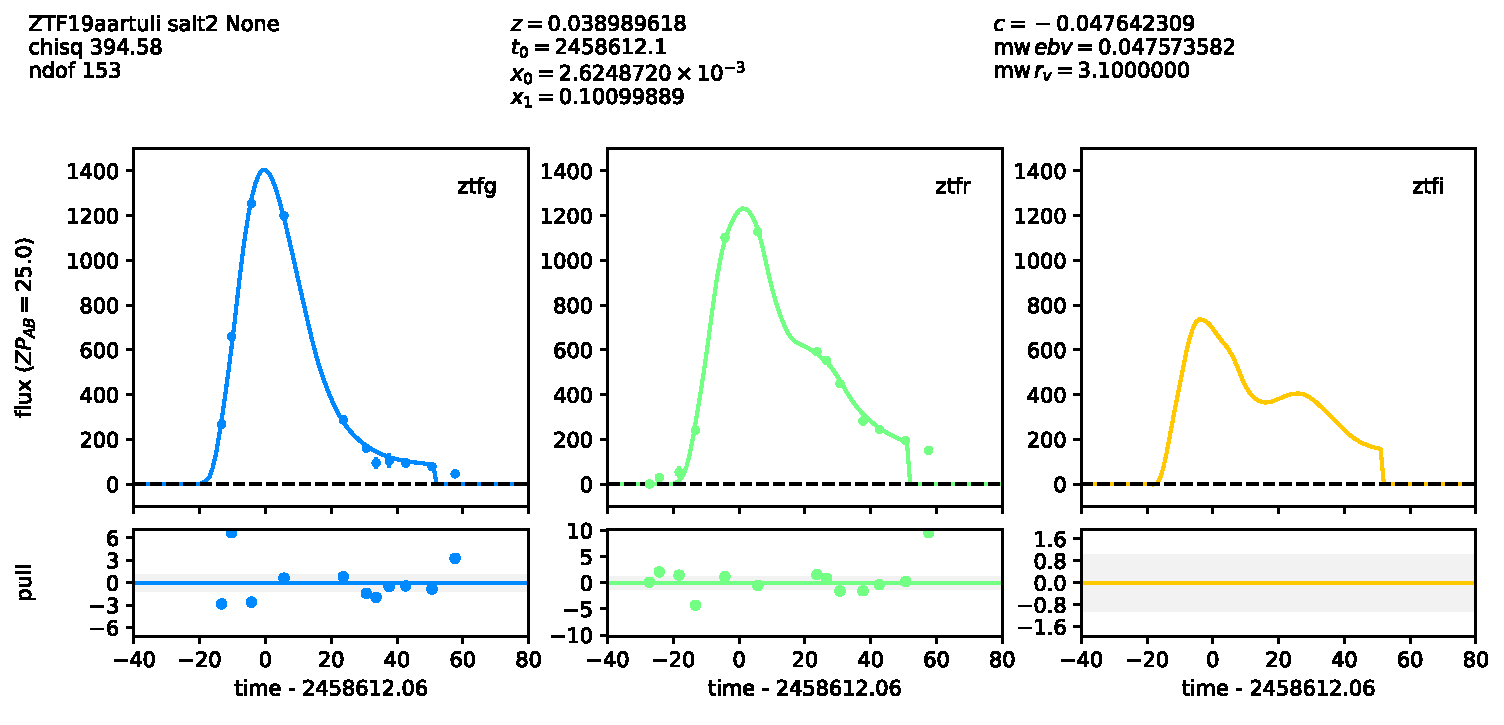
\includegraphics[width=1\textwidth]{nuclear/salt.pdf}
  \caption[SALT2 Fit]{Examplary SALT2 fit output. The three panels show three ZTF bands. Time 0 is the fitted peak of the assumed SN Ia; and as one can see the transient in question is fairly well approximated by SN Ia light curve, with a reduced  $\chi^2=2.67$. The transient is in a fact a spectroscopically classified supernova Ia.}
  \labfig{salt2}
\end{figure}

The fits were performed with \texttt{SNCosmo}, which itself fit the light curve using \texttt{iminuit/MIGRAD}.

\section{Creating Features: Optical Flare Analysis}\label{bayesian_blocks}
Another feature which will later be used in the classification of transients are \textbf{simultaneous flares} across the well-sampled ZTF \textit{g}- and \textit{r}-bands. The number and timing of optical flares within different bands can then be used to differentiate between different types of transients.

\subsection{Bayesian Block Algorithm}\label{bayesian_block}
To determine time periods of heightened activity, a Bayesian block algorithm was employed. This was a version of a package developed at DESY, modified by the author to analyze optical ZTF light curves instead of infrared \textit{WISE} data.

The Baysian Block algorithm is explained in~\sidecite{Scargle1998}; the implementation used here is integrated in the \texttt{astropy} package. The light curves are first smoothed by calculating the median and standard deviation within a 10 day rolling window. After that, only data points lying within $3 \sigma$ distance in magnitude space from the median are used. This gets rid of flux outliers, which are quite frequent for the forced photometry light curves of the nuclear sample.

The prior used for the Bayesian Block analysis was $10 \times \log(n_\text{data})$, with $n_\text{data}$ being the number of datapoints in the smoothed single-band light curve. These numbers were determined empirically to yield robust results. They are a compromise between sensitivity to flux changes and detecting too many, too small blocks to be meaningful.

\subsection{Block Coincidence}
As they are much better sampled than the \textit{i}-band, the \textit{g}- and \textit{r}-band are used to check for blocks temporally coincident in both bands.

For this, each region with increased flux compared to a baseline in the \textit{g}-band is checked to see if there is a corresponding \textit{r}-band block with increased flux overlapping in time.

\begin{figure}
  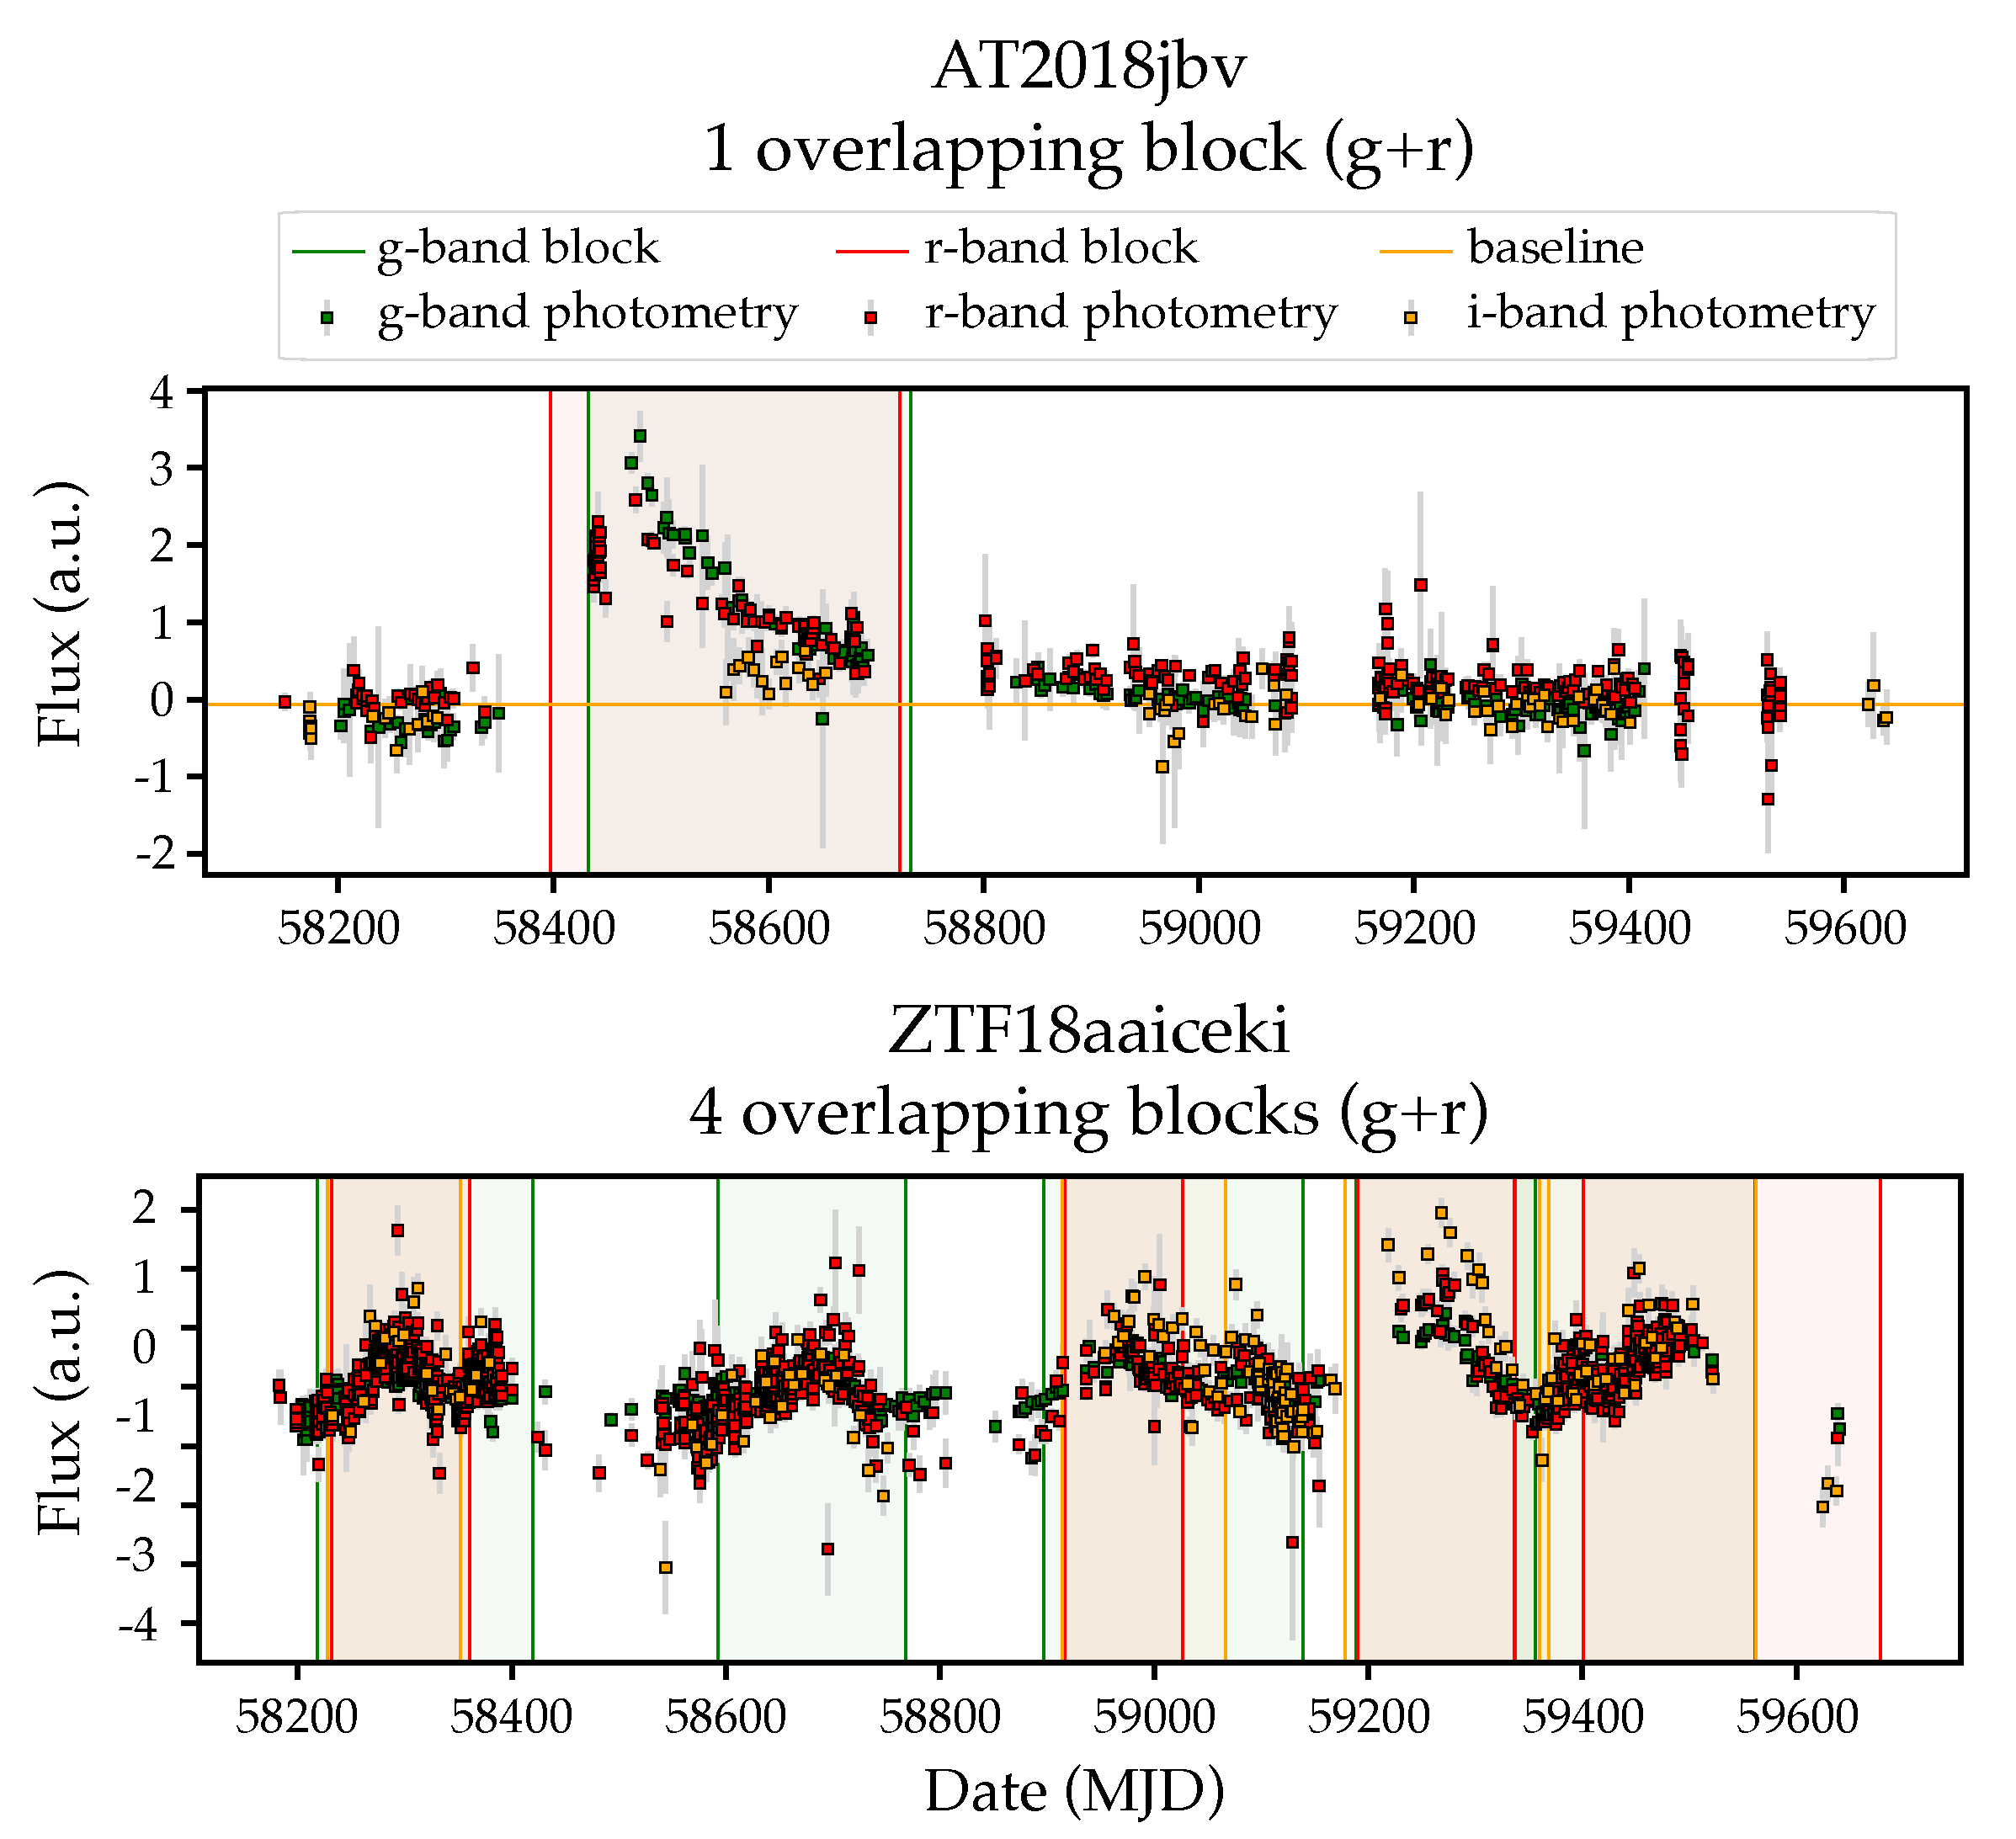
\includegraphics[width=1\textwidth]{nuclear/bayesian_blocks.pdf}
  \caption[Bayesian blocks]{\textbf{Top}: Bayesian Blocks identified for \textit{AT2018jbv}. There is one block both in \textit{g}- and \textit{r}-band, which overlaps. This is a strong indicator that the transient is a one-time flare, stemming from e.g.~a supernova or a TDE (the transient is in fact a TDE), in contrast to stochastic AGN variability. \textit{Bottom}: Bayesian Blocks for \textit{ZTF18aaiceki}, showing AGN activity. This is correctly captured by a large number of overlapping regions.}
  \labfig{bayesian_blocks}
\end{figure}

One can see two examples of such overlapping blocks in Fig.~\ref{fig:bayesian_blocks}, which shows the result of the Bayesian Block algorithm for \textit{AT2018jbv} and \textit{ZTF18aaiceki}. Both are transients from the nuclear sample, the first one being a TDE, the second an AGN displaying stochastic variability.

\section{Training Sample}
As one of the goals is the machine-based classification of the nuclear sample, a training sample that most closely resembles the target sample --- the nuclear sample --- in brightness.

\begin{marginfigure}
  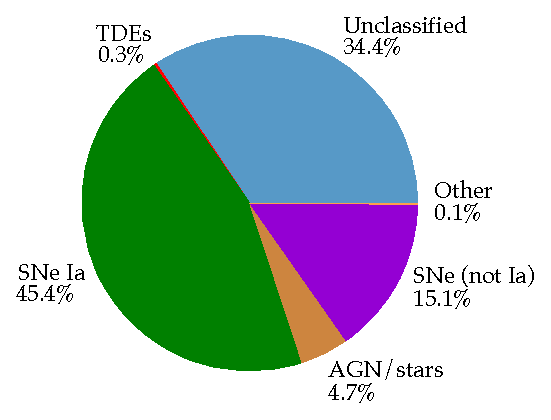
\includegraphics{nuclear/BTS_full.pdf}
  \caption[BTS Composition]{Composition of the Bright Transient Survey sample used in this study. The classified part of the sample is heavily biased towards SNe Ia, AGN are vastly undersampled.}
  \labfig{bts_composition}
\end{marginfigure}

\subsection{The Bright Transient Survey}\label{bts}
The natural starting point for the creation of a training sample was the so-called ZTF Bright Transient Survey (BTS)\sidenote{\url{https://sites.astro.caltech.edu/ztf/bts/bts.php}}, see~\cite{Fremling2020,Perley2020} for details. The basic goal of the survey was spectroscopic classification of all ZTF-detected transients brighter than 18.5 mag in either the \textit{g}- or \textit{r}-band. It even pushes further, achieving a spectroscopic completeness of \SI{75}{\percent} at 19 mag (\SI{93}{\percent} at the nominal cutoff of 18.5 mag)~\cite{Perley2020}.

This was achieved by utilizing the fully robotic SED machine for quick classification, and employing other spectroscopic resources for ambiguous results. BTS is the largest spectroscopic supernova survey ever conducted, with over 8000 classified transients so far (August 2023).

There are three potential issues that need to adressed though when using the BTS as starting point for a training sample:

\begin{description}
  \item[Brightness bias] The BTS restriction to objects usually brighter than 18.5 mag means that the majority of the BTS sample will be brighter than the nuclear sample with its magnitude cut of 20.
  \item[Class imbalance] The BTS is heavily skewed towards supernovae. Also, because SNe Ia are brighter, the majority of the SNe contained in a flux-limited sample like the BTS will be of Type Ia~\cite{Perley2020}. Almost \SI{70}{\percent} of all classified BTS transients are SNe Ia.
  \item[Anti-AGN bias] To reduce contamination stemming from AGN variability, the BTS vetoes transient host galaxies that likely harbor an AGN. This is achieved by crossmatching candidate sources to known AGN, based on \textit{WISE} color cuts, or by rejecting sources with previous variability most likely hinting at AGN activity. As the nuclear sample will contain
\end{description}

These issues need to be solved somehow. Two procedures will be described below: \textbf{Augmentation} by creating fainter copies addresses the brightness bias and partially the class imbalance, while \textbf{either rejecting likely AGN} within the nuclear sample or \textbf{expanding the training set} with known AGN deals with the anti-AGN bias.

\subsection{Augmentation: Enhancing the training set}\label{noisification}
One promising strategy is to multiply the number of light curves available by simulating observations of the same object at higher redshifts.

The method of augmentation employed here was developed by A. Townsend, with significant contribution by the author. The procedure was implemented as Python package~\sidecite{Reusch2023c} and works as follows:

\subsubsection{Draw new redshift}
Obtain a transient light curve (from now on: parent light curve) and parent redshift $z_\text{parent}$ (all classified BTS transients have a spectroscopic redshift).\textbf{Draw a new redshift} $z_\text{child}$ for the child light curve (i.e. the noisified copy) from a cubic redshift distribution ranging from $z­_\text{parent}$ to $z_\text{parent}+0.1$.

\subsubsection{Scale and scatter the flux}
After this, \textbf{the parent flux was redrawn} from a normal distribution centered around each parent flux value, scaled by its error. This was done to account for the fact that flux measurements are expected to scatter around their true value with their error, thereby simulating a `new' measurement. After this, the re-drawn flux measurements were rescaled with the new redshift $z_\text{child}$. The flux $F$ scales according to $D_L=\frac{L}{4 \pi F}$ i.e.~with the square of the luminosity distance (see Section~\ref{fitmodels}). Therefore, one can determine a \textbf{flux scaling factor} $a$ according to
\begin{equation}
  a = \frac{D_L(z_\text{parent})^2}{D_L(z_\text{child})^2}.
\end{equation}
With this scaling factor, the child lightcurve flux is simply $f_\text{child} = a f_\text{parent}$.

The flux error gets scaled accordingly, but with two additional empirical constant coefficients $e_f$ and $e_b$ determined by fitting the flux error as a function of flux. This procedure showed that the error $F_\text{err}$ deviates from the expected $\sqrt{F}$ behavior, but can be well approximated by $F_\text{err} = \sqrt{F + e_f^2\times F + e_b^2}$. The error as a function of flux, as well as the different approximations are shown in Fig.~\ref{fig:ztf_error_dist}. The factors $e_f$ and $e_b$ were determined as $e_f = 0.54$ and $e_b = 5.37$.

\begin{marginfigure}
  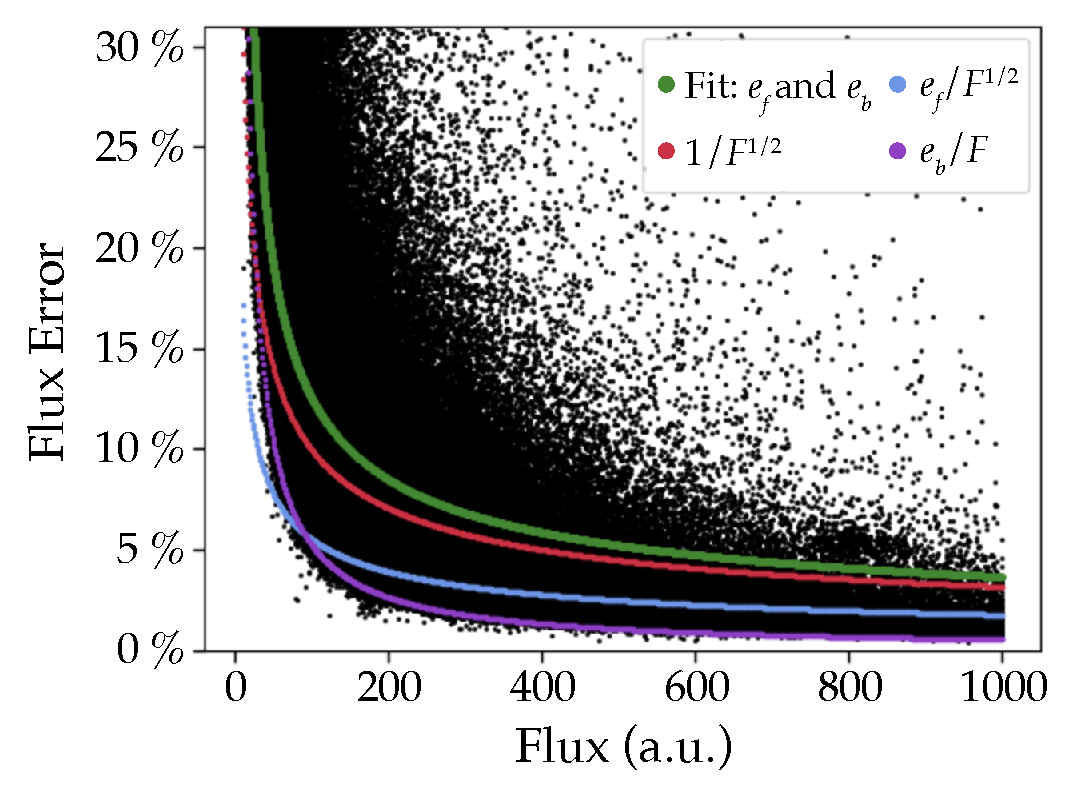
\includegraphics{nuclear/ztf_error_dist.pdf}
  \caption[ZTF error distribution]{ZTF error distribution: $F$ vs. $F_\text{err}$ in percentage of flux. The red curve shows the expected error behavior ($F_\text{err}\propto \sqrt{F})$, while the green curve shows the improved version $F_\text{err} = \sqrt{F + e_f^2\times F + e_b^2}$. Figure by A. Townsend with small modifications by the author.}
  \labfig{ztf_error_dist}
\end{marginfigure}

\subsubsection{Apply K-Correction}
If an \texttt{SNCosmo} model for the transient type did exist, \textbf{K-correction} was applied. This procedure accounts for the fact that by arbitrarily redshifting the light curve of an object, the spectrum will also be redshifted. Due to this, the bandpasses will register different parts of the spectrum, which leads to a different observed flux (see~\sidecite{Hogg2002} for an introduction).

\subsubsection{Scatter observations}
As a last step, the created light curve is sampled with a default retention fraction of 0.9, i.e.~\SI{10}{\percent} of data points are randomly dropped. Additionally, the observation times are slightly randomized to avoid creating regularities a machine-learning algorithm could pick up. This is achieved by scattering the observation dates around their original values, with a $\sigma$ of $0.03$ days.

\subsubsection{Reject faint light curves}
Finally, for each generated light curve, at least 5 datapoints were required to \textbf{lie above a detection threshold} of $5 \sigma$. If that requirement was not met, the light curve was discarded. This was implemented to mimic the nuclear filter (see Section~\ref{nuclear_filter}), which reacts to alerts issued by ZTF. Only datapoints with a signal-to-noise ratio of $>5$ warrant an alert, so the noisified light curves need at least some datapoints above that threshold. The minimal number of detections for the noisified light curves is a bit higher compared to the nuclear filter (5 vs. 3) to account for the fact that forced photometry is slightly more sensitive than the PSF photometry used in the alerts.

\subsubsection{Sample dynamically}
Depending on the number of light curves for a specific class, the number of desired child light curves per parent light curve was determined to yield a noisified training set with balanced classes. For example, only 3 children per SN Ia light curve were generated, but up to 14 children per light curve of all other types of supernovae. The only exception were variable stars: For these, the redshift $\approx 0$ and could not be varied, so no noisified children were generated.

The results of all these steps are exemplified in Fig.~\ref{fig:noisify_example}. It shows the light curve of a SN Ia, \textit{SN2019qym}, detected with a redshift of $z=0.02$. The original light curve can be seen, as well as a noisified child light curve at higher redshift ($z=0.09$). Note the increase errors (the original object was very bright, so only one datapoint in the \textit{g}-band at 35 days after peak has visible error bars), the slighty different modified observation dates and the random removal of datapoints.

\begin{figure}[H]
  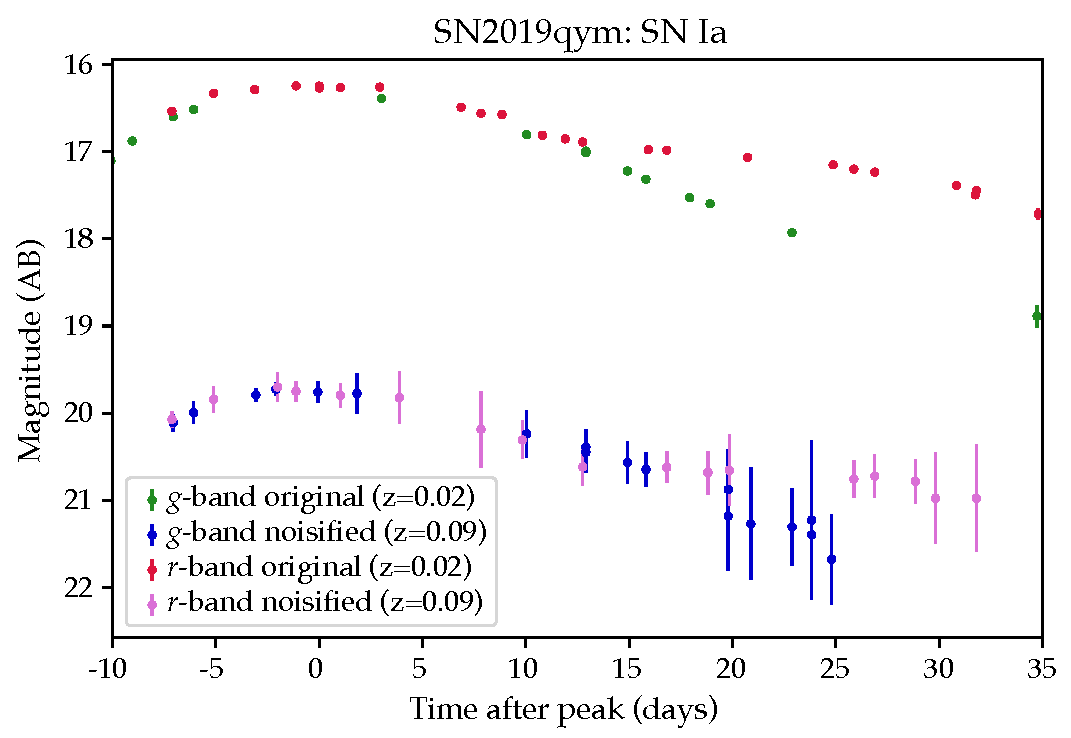
\includegraphics[width=1\textwidth]{nuclear/noisify_ZTF19acapeun.pdf}
  \caption[Augmentation example]{Original and `child' light curve of \textit{SN2019qym}, a SN Ia with a redshift of $z=0.02$. The original two bands are shown in green and red, while the fainter, noisier copy at a redshift of $z=0.09$ is displayed in blue and pink. Figure by A. Townsend, with slight modifications by the author.}
  \labfig{noisify_example}
\end{figure}

\subsection{AGN Rejection}\label{agn_rejection}
To match the anti AGN-bias within the BTS, in principle two methods are available: Increase the number of AGN in the training sample, or veto against AGN in the sample that needs classification.

The latter approach was chosen here, so only those nuclear transients that survived the AGN rejection were kept for classification. The AGN rejection was performed as a two-step process, based on \text{WISE}-colors and matches to the Milliquas catalog.

\subsubsection{\textit{WISE} color selection}\label{wise_color_cut}
The cuts applied were taken from~\cite{Hviding2022}. The authors evaluated roughly half a million SDSS galaxies with matching \textit{WISE} infrared data, resulting in a region within the \textit{WISE} color-color diagram that robustly picks out AGN. The AGN `box' is defined as follows:
\begin{subequations}
  \begin{eqnarray}
    1.734 < (\textit{W2}-\textit{W3}) < 3.916 \\
    (\textit{W1}-\textit{W2}) > 0.0771 (\textit{W2}-\textit{W3}) + 0.319 \\
    (\textit{W1}-\textit{W2}) > 0.261 (\textit{W2}-\textit{W3}) - 0.260.
  \end{eqnarray}
\end{subequations}
All objects lying within this box (dot-dot-dashed contours in Fig.~\ref{fig:agn_box}) were rejected as likely AGN.

\begin{figure}[htpb]
  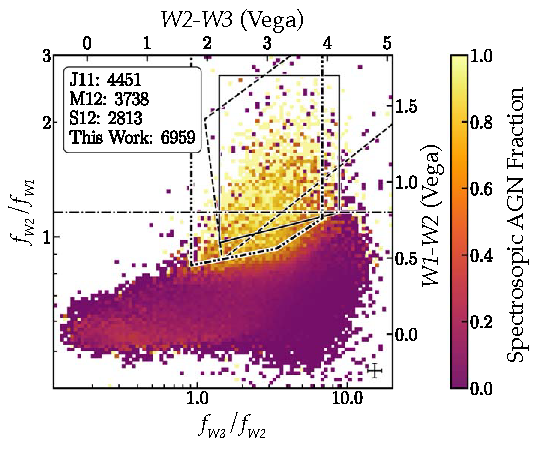
\includegraphics[width=0.8\textwidth]{nuclear/agn_box.pdf}
  \caption[Infrared AGN selection]{AGN Selection based on infrared \textit{WISE} colors. It shows the \textit{W2}-\textit{W3} vs. \textit{W1}-\textit{W1} color; the fraction of spectroscopically classified AGN is encoded in datapoint color. The dot-dot-dashed box is the one used to flag likely AGN. Adapted from~\cite{Hviding2022}.}
  \labfig{agn_box}
\end{figure}

\subsubsection{Milliquas matching}\label{milliquas_cut}
Additionally to the \textit{WISE} color selection, the Milliquas~\cite{Milliquas} catalog~\sidenote{\url{https://quasars.org/milliquas.htm}} was also used to identify likely AGN. This catalog was also used in the regular high-energy neutrino follow up (see Section~\ref{catmatch}). It contains over 900,000 Type I AGN, roughly 50,000 Type II AGN and again as many quasar candidates.

As we were interested in maximizing the purity of the sample in terms of AGN, i.e.~rejecting all likely AGN. Therefore, all objects that had a match in the Milliquas catalog --- no matter the likelihood of the match being an AGN --- were rejected.

\subsection{Adding non-BTS Sources}\label{addsources}
As one of the desired features of the trained classifier was its ability to correctly identify TDEs, it was necessary to incrase the number of TDEs in the training sample. For reasons not accessible to the author, the BTS underperformed significantly in terms of TDE detection rate.

To augment the training sample, all published ZTF-detected TDEs were also included. In total, these amounted to 65 events.

To counter the fact that almost no AGN were present in the BTS sample, forced photometry for an additional 1772 AGN light curves was acquired. This was done by crossmatching sources from a recent AGN study including redshifts~\sidecite{Mechbal2023} with ZTF alerts in a cone with a radius of 3 arcsec.

\subsection{Creating a less biased Training Sample}
It was not fully possible to control the number of noisified child light curves: There were cases of low-flux objects of which all noisified children failed the signal-to-noise cut. In total, the following number of objects were processed during the training sample augmentation:
\begin{description}
  \item[SNe Ia] The BTS contained 3230 SNe Ia, from which 8694 nosified children were created,~i.e. 2.7 children per original light curve on average. The total number of light curves (original ones plus children) was 11924.
  \item[Core-collapse SNe] 1075 CCSNe were available in the BTS. With an average of 10.6 children per light curve this amounted to 11420 noisified children and 12495 light curves in total.
  \item[AGN] 1893 AGN were originally present. 7177 children were created (3.8 per parent), resulting in 9079 light curves.
  \item[TDE] Starting with 66 TDE, 13097 children were creating with a large number of children per light curve (198). This amounted to 13163 light curves in total.
  \item[Stars] As already stated above, stars were not noisified due to their redshift being practically 0. Therefore, only the 525 parent light curves were used, rendering stars the most underrepresented class within the training sample.
\end{description}
Overall, the final training sample contained 47186 light curves, generated from 6789 initial light curves. On average, $~\sim 6$ child light curves were creates from each parent.

\section{Training the Model}
In recent years \texttt{XGBoost}\sidenote{\url{https://xgboost.ai}}~\sidecite{Chen2016}, an optimized gradient-boosted decision tree algorithm (this will be explained below), has performed well when classifying structured data.

\subsection{Boosted Decision Trees}
In a regular \textbf{decision tree}, a set of iterative binary decisions (hence `tree') are employed to decide on the classification of an object. \textbf{Ensemble methods} build upon this concept by either working in parallel by creating multiple decision trees with random subsets of features (\textbf{random forest}) or by working in sequence. The latter method qualifies \textbf{boosted} decision trees, meaning that decision trees are generated and evaluated in sequence. The residual squared errors from the first tree are fed into the second tree, and so on. The final classification then is the (weighted) sum of all individual tree's classifications. This method can be generalized to differentiable loss functions in general. If one uses the negative gradient of the squared error loss function instead of the squared error itself, the algorithm is called \textbf{gradient boosting}. \texttt{XGBoost} is one variant of such a gradient boosting algorithm.

\subsection{Hyperparameter Search}
As is usual with such algorithms, there is a number of \textbf{hyperparameters} which determine how \texttt{XGBoost} behaves. \texttt{max\_depth} for example avoids overfitting by restricting the size of individual decision trees, the \texttt{learning\_rate} scales down the results by trees which are not the first one, and \texttt{n\_estimators} controls the number of trees.

These hyperparameters can be tuned by running a \textbf{grid search} in the parameter space, each time training with a small subset of the full data to speed up the process. The parameters yielding the best result are then used when training the full model with the complete training set. In this work, the best values for 9 hyperparameters were searched by randomly drawing from a grid of parameters combinations for 5000 times. This was chosen as a compromise between computational feasibility and optimizing the parameter set. The grid employed as well as the chosen hyperparameters are shown in the appendix in Table~\ref{tab:xgboost_grid_search}.

\subsection{Training Procedure}
After obtaining a classified training sample (BTS light curves, see Section~\ref{bts}), AGN and TDE light curves were added (Section~\ref{addsources}) and the sample was augmented and enlarged by creating redshifted and noisified copies (Section~\ref{noisification}). After this, the full training sample was fit with SALT2~(Section~\ref{salt}) and a TDE model (Section\ref{tde_model}), as well as analyzed with a bayesian block algorithm (Section~\ref{bayesian_blocks}) to extract features.

The set of features used for training was the following:

\begin{description}
  \item[Peak magnitude] This is the peak observed magnitude (in any filter). The value was scaled accordingly for the noisified and redshifted child light curves:
    \begin{subequations}
      \begin{eqnarray}
        m_\text{child} &=& m_\text{parent} - \mu­_\text{parent} + \mu_\text{child}~~\text{and}\\
        \mu &=& 5(\log_{10}D_L(z)+1),
      \end{eqnarray}
    \end{subequations}
    where $m$ is the parent or child magnitude, $\mu$ is the distance modulus, and $D_L$ is the luminosity distance for redshift $z$.
  \item[SALT2 Fit Results] This included SALT2 fit parameters $x_0$, $x_1$ and $c$, as well as the reduced $\chi^2$, the non-reduced $\chi^2$ and the degrees of freedom.
  \item[TDE Fit Results] The best-fit TDE Model parameters were also included. These were the rise- and decay times, the peak temperature, the temperature change and the amplitude. The temperature change cutoff time was not included, as the model never picked on this parameter. The results also included the $\chi^2$ and degrees of freedom.
  \item[Overlapping blocks] The number of overlapping regions, extracted with the bayesian block analysis, was also included to allow identification of non-repeating flares (in contrast to stochastic AGN behavior).
  \item[\textit{WISE} colors] To identify likely AGN, the \textit{WISE} \textit{W1}-\textit{W2} and \textit{W2}-\textit{W3} colors of the parent host were also added.
  \item[\texttt{sgscore}] The \texttt{sgscore} of the parent light curve, based on machine learning with PS1 photometry (see Section~\ref{ztf_image_subtraction}), is included as a proxy for host galaxy photometry and morphology.
  \item[Core distance] The median core distance was also included. To account for the fact that the core distance of the redshifted child light curves will change with respect to their parents, this value was recalculated for all children. This was done according to
    \begin{equation}
      \theta_\text{child} = \theta_\text{parent} \frac{D_L(z_\text{parent})}{D_L(z_\text{child})} \frac{(1+z_\text{child})^2}{(1+z_\text{parent})^2},
    \end{equation}
    where $\theta$ is the angular core distance of the child or parent light curve, $D_L$ is the luminosity distance and $z$ is the respective redshift.
\end{description}

\section{Evaluating the Model}
A large fraction of the nuclear sample was unclassified --- this is why we a classifier was needed in the first place. Therefore, evaluating the classifier's performance needed to happen with a part of the BTS training set. This was done in the usual way: \SI{30}{\percent} of the training set was kept aside, never to be seen by the classifier beforehand. Such a sample is called a \textbf{test set}.

\subsection{Strict Separation of Training and Test}
One pitfall needs to be avoided: The model might learn features of a noisified test light curve by having already seen its parent or one of its siblings in the training process, thereby cheating. To deal with this, the parent light curve and all of its children were always kept together: If e.g.~one child light curve was part of the training set, so were its parent and all its siblings.

\subsection{Performance}
We are now ready to see how the model performs. This is done by first investigating the feature importance, and then by evaluating the confusion matrices.

\subsubsection{Feature Importance}
As one can see in Fig.~\ref{fig:feature_importance}, the feature importance looks decent. There is not one dominating feature, which would be indicative of the classifier finding a loop hole regarding the actual task. There are also no features that do not influence the classification at all.

\begin{figure}[htpb]
  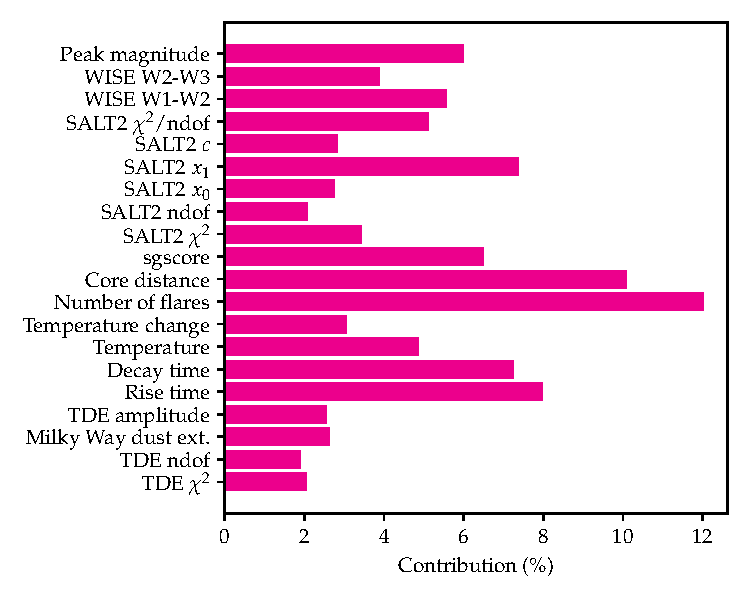
\includegraphics[width=0.6\textwidth]{nuclear/confusion/feature_importance_niter_5000_nsample_2000.pdf}
  \caption[Feature importance]{Feature importance for the classifier when trained with the augmented BTS sample.}
  \labfig{feature_importance}
\end{figure}

The two most important features are the TDE fit rise- and decay time, followed by the SALT2 fit $x_1$ parameter\todo{not true}, which encodes the stretch of the light curve. The \textit{WISE} colors are also signficant, as the classifier probably captures the importance of \textit{WISE} colors for AGN classification.

Unfortunately, the temperature and temperature change do not seem to play a major role. This is indicative of the TDE model fit not capturing all physically present information. It has been shown that (missing) light curve color evolution is a good predictor for TDEs (see e.g.~\cite{Velzen2021a}). As the blackbody temperature and temperature change should in principle encode color evolution, it is somewhat surprising that these two features do not mirror the importance of color information.

\subsubsection{Confusion Matrices}\label{confusion_matrices}
To see how the model performs with regards to the test set, one could either evaluate a version of the test set also containing noisified light curve children, or only parent light curves. There was no reason to favor one over the other, so both evaluations were done.

\subsubsection{Test without Noisified Light Curves}
The results from only allowing `real' light curves (i.e.~parent light curves) can be seen in Fig.~\ref{fig:confusion_nonoise}.

\begin{figure}[htb]
  \centering
  \begin{subfigure}[b]{0.49\textwidth}
    \centering
    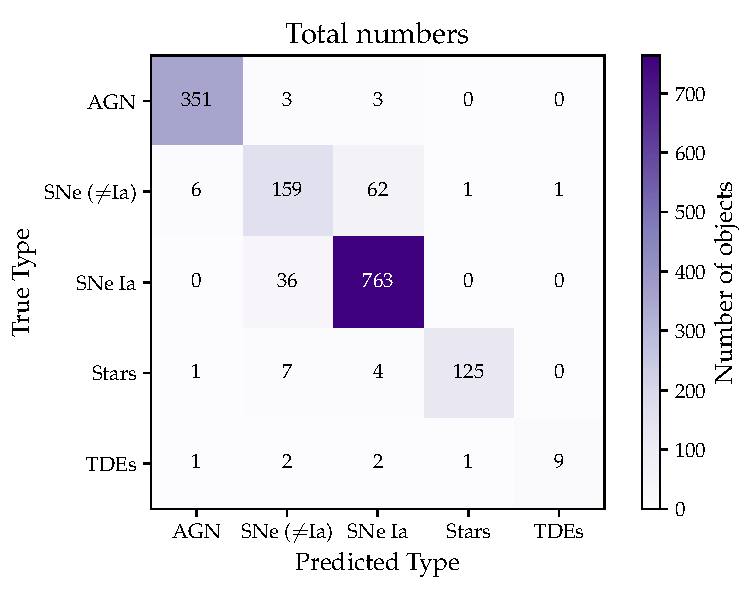
\includegraphics[width=1\textwidth]{nuclear/confusion/results_seed_10_n_iter_5000_noisified_val_False_normaliz_None.pdf}
  \end{subfigure}
  \begin{subfigure}[b]{0.49\textwidth}
    \centering
    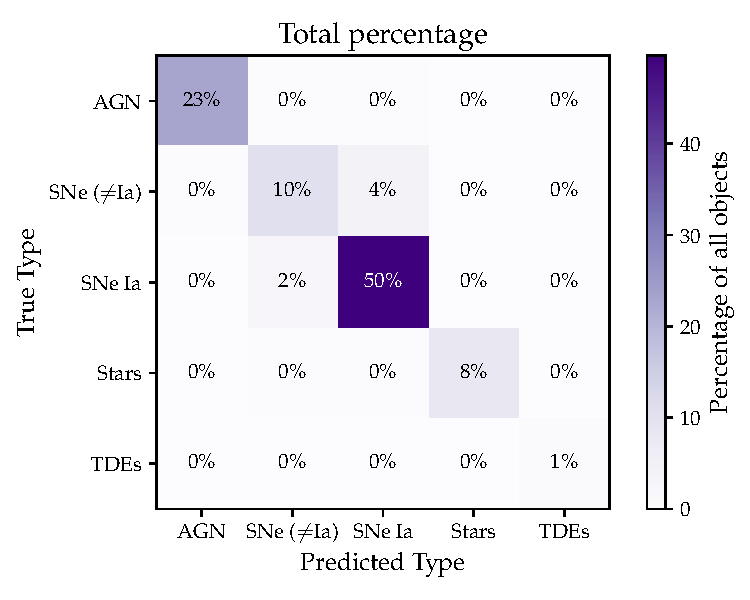
\includegraphics[width=1\textwidth]{nuclear/confusion/results_seed_10_n_iter_5000_noisified_val_False_normaliz_all.pdf}
  \end{subfigure}
  \begin{subfigure}[b]{0.49\textwidth}
    \centering
    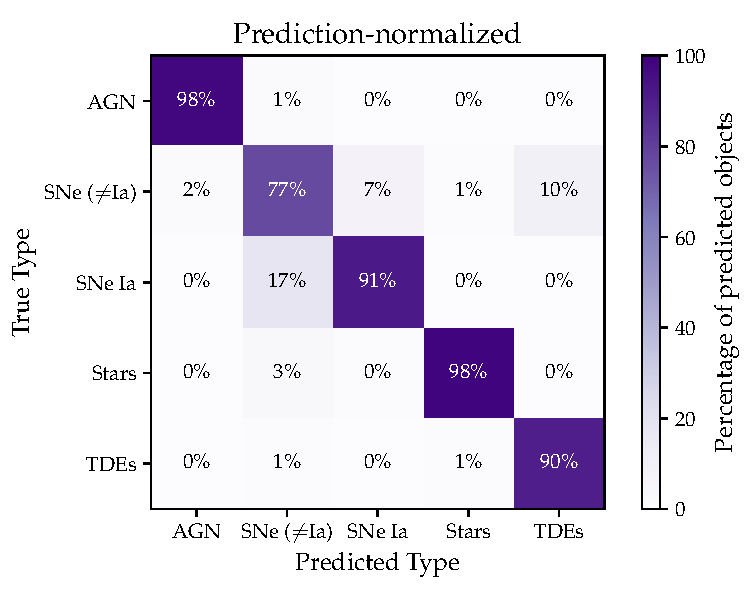
\includegraphics[width=1\textwidth]{nuclear/confusion/results_seed_10_n_iter_5000_noisified_val_False_normaliz_pred.pdf}
  \end{subfigure}
  \begin{subfigure}[b]{0.49\textwidth}
    \centering
    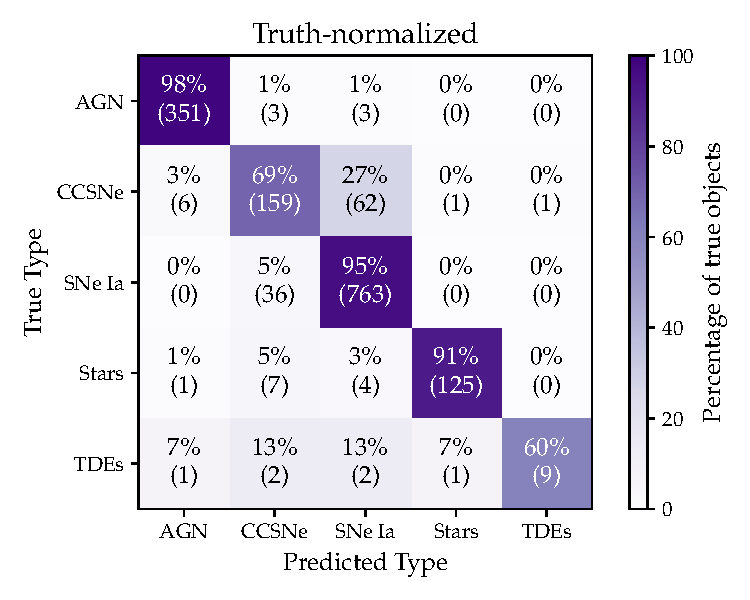
\includegraphics[width=1\textwidth]{nuclear/confusion/results_seed_10_n_iter_5000_noisified_val_False_normaliz_true.pdf}
  \end{subfigure}
  \caption[Confusion matrices without augmentation]{Confusion matrices of the test set predictions, \textbf{excluding} noisified light curves. For each figure, the row corresponds to the true type, and the column to the predicted type of object. The matrix on the top left shows the total numbers, while all other matrices show percentage. The bottom left matrix shows prediction-normalized values, while the bottom right matrix shows truth-normalized values.}
  \labfig{confusion_nonoise}
\end{figure}

As one can see in the top right plot, when exluding noisified light curves, the test set is naturally heavily biased towards SNe Ia as well (like the training set), and only 16 TDEs are present.

The bottom left matrix shows the \textbf{prediction-normalized} values: Each number is the percentage of the predicted classifications actually belonging to the predicted class. For example, \SI{90}{\percent} of all predicted TDE are actually TDE, the other \SI{10}{\percent} are CCSNe in truth. In short, these \SI{10}{\percent} are the false positive rate.

The \textbf{truth-normalized} matrix (bottom right) shows the percentage with which objects that in truth belong to a class are correctly identified as class members. \SI{60}{\percent} of all TDE were correctly identified as TDE, but \SI{7}{\percent} were misclassified as AGN, \SI{13}{\percent} were wrongly identified as SNe Ia, \SI{13}{\percent} as CCSNe, and \SI{7}{\percent} as stars. The sum of all misclassifications, in this case \SI{40}{\percent} correspond to the false negative rate for TDE classification.

The \textbf{performance looks quite decent, especially the false positive rate}: Except for CCSNe, all predictions capture the truth in \SI{\geq90}{\percent} of all cases. Also, the \textbf{TDE identification seems to work fairly well}, with \SI{60}{\percent} of all TDEs identified by the classifier as such, of the 10 objects predicted to be TDEs, only 1 was not a TDE. The validity of this result is of course limited by the small number of TDEs in the test sample. As the number of available ZTF light curves of confirmed TDEs is only in the double digits, there is no easy fix to this problem.

\subsubsection{Test with Noisified Light Curves}
The evalation above was repeated, but this time \textbf{including noisified child light curves}. The results can be seen in Fig.~\ref{fig:confusion_noise}.

The sample looks more balanced due to the inclusion of more noisified child light curves for underrepresented classes (except stars). As one would expect, the overall performance does increase when compared to the test set without child light curves: \SI{97}{\percent} of all predicted TDEs were in fact TDEs (compared to \SI{90}{\percent} without noisified light curves in the test set), and \SI{79}{\percent} of all TDEs were identified as such (no noisified test: \SI{60}{\percent}).

\begin{figure}[htb]
  \centering
  \begin{subfigure}[b]{0.49\textwidth}
    \centering
    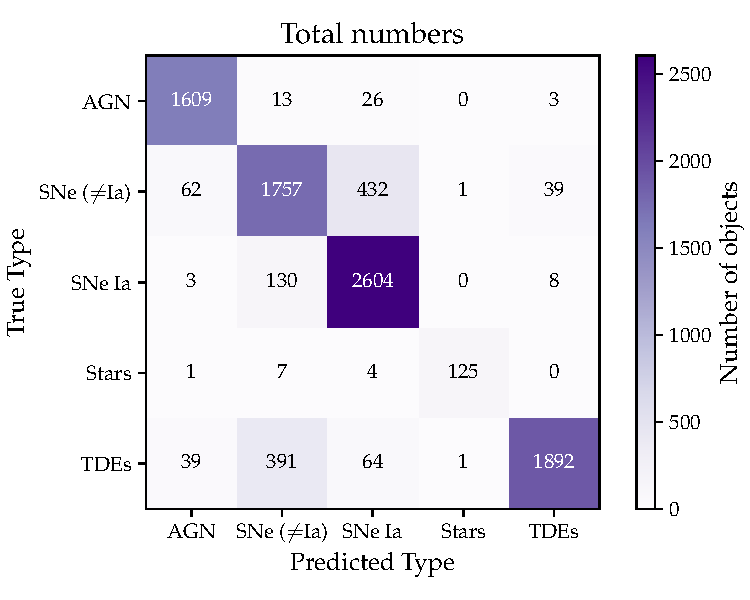
\includegraphics[width=1\textwidth]{nuclear/confusion/results_seed_10_n_iter_5000_noisified_val_True_normaliz_None.pdf}
  \end{subfigure}
  \begin{subfigure}[b]{0.49\textwidth}
    \centering
    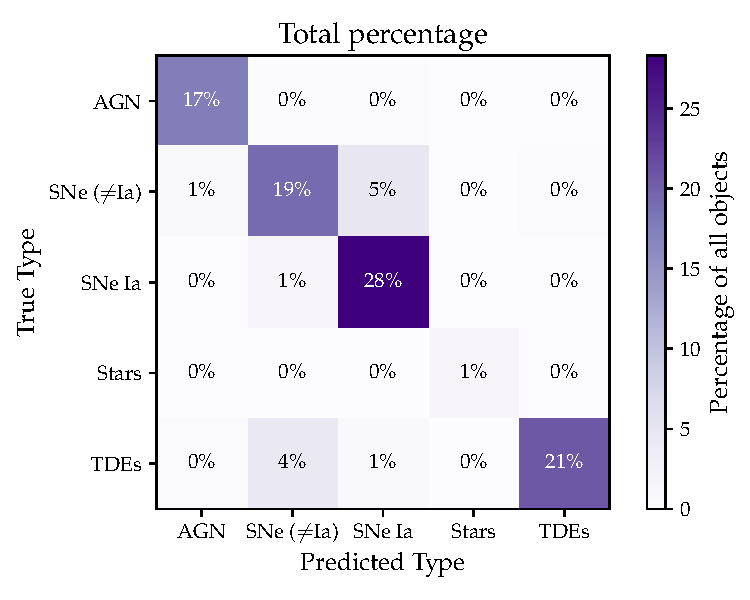
\includegraphics[width=1\textwidth]{nuclear/confusion/results_seed_10_n_iter_5000_noisified_val_True_normaliz_all.pdf}
  \end{subfigure}
  \begin{subfigure}[b]{0.49\textwidth}
    \centering
    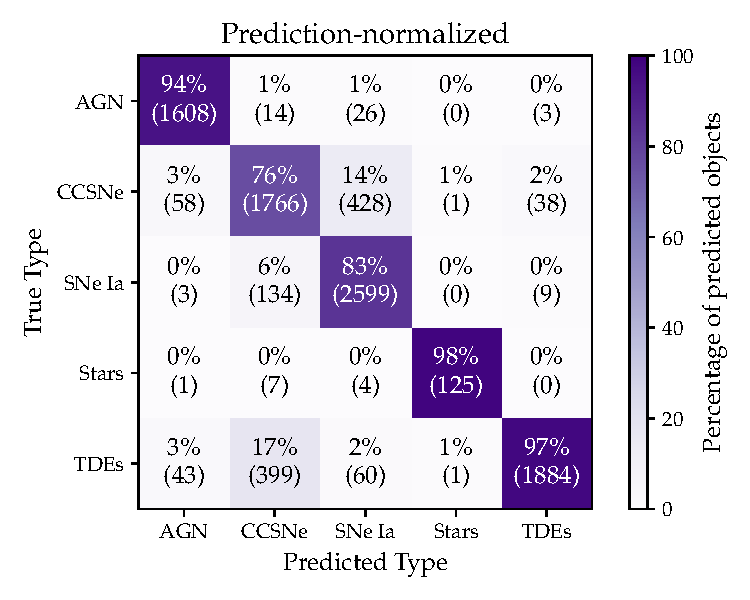
\includegraphics[width=1\textwidth]{nuclear/confusion/results_seed_10_n_iter_5000_noisified_val_True_normaliz_pred.pdf}
  \end{subfigure}
  \begin{subfigure}[b]{0.49\textwidth}
    \centering
    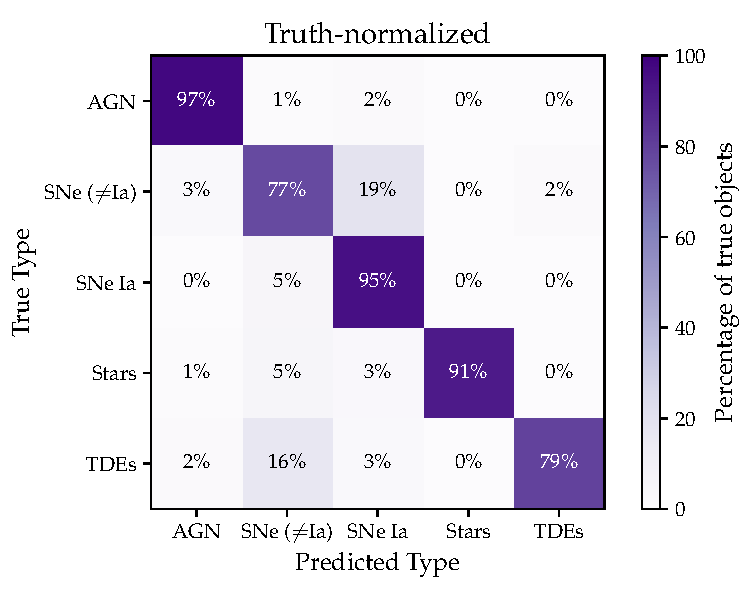
\includegraphics[width=1\textwidth]{nuclear/confusion/results_seed_10_n_iter_5000_noisified_val_True_normaliz_true.pdf}
  \end{subfigure}
  \caption[Confusion matrices with augmentation]{Confusion matrices of the test set predictions, \textbf{including} noisified light curves. Top left: total numbers; top right: total percentages; bottom left: prediction-normalized; bottom right: truth-normalized.}
  \labfig{confusion_noise}
\end{figure}



% Nevertheless, both the evaluation without and with noisified child light curves carry meaning. The latter is less affected by small sample statistics, while the former 
%  probably more meaningful, as \todo{why}

\section{Finding Candidate TDEs}\label{visual_cuts}
% Besides a full classification of the nuclear sample, another purpose of the classifier was to obtain a \textbf{selection of candidate TDE with high purity}.
% Finally, we 

The traditional method of selecting TDE candidates is comprised of a sequence of \textbf{visual cuts} in the fit result parameter space (see e.g.~\cite{Velzen2019}). One way of increasing the purity of the machine-learning selected TDE is by defining such a set of visual cuts by studying the BTS sample, and applying the very same cuts to the nuclear sample.
%  To get a handle on the results of the machine learning classification and \textbf{evaluate the discriminatory power} of the features in an independent way, a similar approach was chosen here.

To do this, the classified part of the BTS sample with additional TDEs added was evaluated with exactly the same features as used in the training of the classifier model. The goal was to look for a set of cuts in the fit parameter space that would retain a high number of TDEs (maximizing efficiency), while rejecting as many non-TDE as possible (maximizing purity).

\subsection{Visual Cuts: Different Cut Stages}
An overview over the sample after subsequent application of these cuts, as well as the TDE selection efficiency and purity can be seen in Figure~\ref{fig:bts_scatter}. These were the stages (the numbers in brackets correspond to the individual plots, with (1a) showing the sample without cuts):

\begin{description}
  \item[AGN Veto (1b, 2a)] Although the BTS is already biased against AGN, the BTS sample still contained objects which could be ruled out as likely AGN by crossmatching to Milliquas (1b) and selecting based on \textit{WISE} colors (2a), see Section~\ref{agn_rejection}.
  \item[Core distance (2b)] As the BTS is not selecting nuclear transients per se, this needed to be enforced by requiring a maximum core distance of 0.4 arcseconds.
  \item[\texttt{sgscore} cut (3a)] Only transients with an \texttt{sgscore} $<0.3$ were allowed in this cut stage.
  \item[SNIa diagonal cut (3b)] The transient had to be to the right side of a diagonal cut in the rise decay time plane, described by $3.55 - 2.29 \tau$ (with $\tau$ being the decay time and everything in $\log~\text{day}$).
  \item[Temperature cut (4a)] The temperature was required to lie between $\log \SI{3.9}{\K}$ and $\log\SI{4.4}{\K}$. Furthermore, the daily temperature change $\Delta T$ was required to lie between $\SI{-100}{\K\per\deh} < \Delta T < \SI{150}{\K\per\deh}$ (left).
  \item[Rise- and decay-time cut (4b)] The rise and decay times were required to lie within $\log \SI{0.8}{\deh} < \text{risetime} < \log \SI{2.05}{\deh}$ and $\log \SI{1.1}{\deh} < \text{decaytime} < \log \SI{3.0}{\deh}$.
  \item[$\chi^2$ cut (5a)] Only those transients with a TDE fit reduced $\chi^2$ outperforming their SALT2 fit reduced $\chi^2$ were selected here to reject remaining likely SNe Ia. Also, the reduced TDE fit $\chi^2$ was required to lie below 6.
  \item[Exactly one flare (5b)] Finally, only transient with a single flare coincident in \textit{g}- and \textit{r}-band were allowed to reject likely stochastic AGN activity.
\end{description}

\subsection{Visual Cuts: Evaluate the Cuts}
Before all cuts, only requiring the TDE model fit to succeed, the sample consists of 4094 transients, of which 64 are TDEs. This corresponded to an initial purity of \SI{1.6}{\percent} and a selection efficiency of \SI{100}{\percent} (all TDEs are of course retained before any cuts).

\subsubsection{All Cuts Combined}
The final selection consisted of 39 transients, of which 31 were TDE. This translates to a purity of \SI{79.5}{\percent}, with a selection efficiency of \SI{48.4}{\percent}, i.e.~roughly half of the TDE survive all cuts.
The efficiency and purity with subsequent cut stages is shown in Fig.~\ref{fig:efficiency_purity}.

\begin{figure}[htpb]
  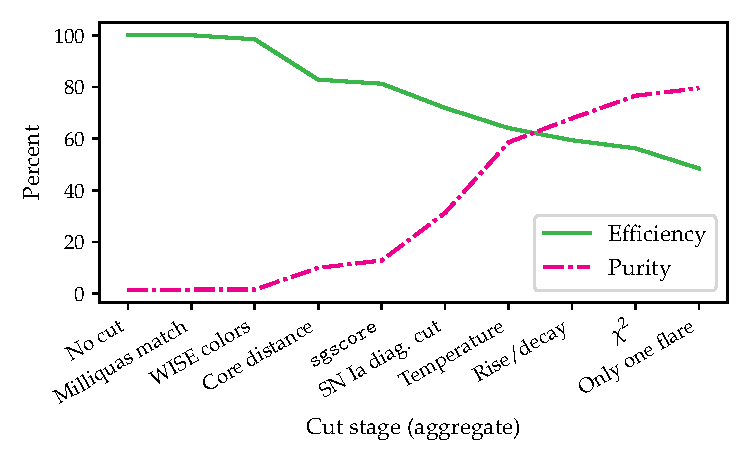
\includegraphics[width=1\textwidth]{nuclear/efficiency_purity.pdf}
  \caption[Visual TDE selection]{Efficiency (green line) and purity (magenta, dash-dot) of the visual TDE selection. The cut stages are shown on the x-axis, with each new cut added on top of all previous cuts.}
  \labfig{efficiency_purity}
\end{figure}

These numbers are somewhat promising, as objects lying within the final selection \textbf{have a 4 in 5 chance of correctly being identified as TDE}, while only sacrificing half the TDE population. Of course, there is always a trade-off between efficiency and purity, and a program designated to maximizing the number of TDEs discovered might accept a lower purity.

\subsubsection{Independent Cuts}
To estimate the individual selection power of the different cuts, these were also applied independently, i.e.~without any other cuts. The results of these individual cuts can be seen in Table~\ref{tab:visual_selection}. When using the ratio between purity gain and efficiency loss as a figure of merit, the \texttt{sgscore} cut is the best. When applied to the nuclear sample though, it will not improve things like here for the BTS sample, as the nuclear sample by construction already includes this cut. The next best ones are the core distance cut (also this is already incorporated in the nuclear sample), and the diagonal rise-decay time based SN Ia cut.  The \textit{WISE} color cut and the Milliquas cut have basically no effect, which is not surprising the heavy bias against AGN of the Bright Transient Survey. The $\chi^2$ and temperature cuts seem to work fine, while the rise-/decay-time based cut and the one flare requirement seem to underperform.

\begin{table}
  \centering
  \def\arraystretch{1.2}
  \begin{tabular}{c c c c c c}
    \hline
    \textbf{Parameter}         & \textbf{Purity} & \textbf{Efficiency} & \textbf{Purity}    & \textbf{Efficiency} & \textbf{Ratio} \\
                               & \textbf{(\%)}   & \textbf{(\%)}       & \textbf{gain (\%)} & \textbf{loss (\%)}  &                \\
    \hline
    \hline
    \textbf{No cut}            & 1.6             & 100                 & 0                  & 0                   & ---            \\
    \textbf{Milliquas cut}     & 1.6             & 100                 & 1.8                & 0                   & ---            \\
    \textbf{\textit{WISE} cut} & 1.6             & 98.4                & 0.7                & 1.6                 & 0.5            \\
    \textbf{Core distance}     & 8.7             & 82.8                & 458.5              & 17.2                & 26.7           \\
    \textbf{\texttt{sgscore}}  & 2.5             & 98.4                & 58.2               & 1.6                 & 37.2           \\
    \textbf{SN Ia Cut}         & 5.2             & 90.6                & 234.9              & 9.4                 & 25.1           \\
    \textbf{Temperature}       & 3.1             & 85.9                & 101.4              & 14.1                & 7.2            \\
    \textbf{Rise-/Decay}       & 2.4             & 84.4                & 52.0               & 15.6                & 3.3            \\
    \textbf{$\chi^2$}          & 3.6             & 92.2                & 127.4              & 7.8                 & 16.3           \\
    \textbf{One flare}         & 2.2             & 82.8                & 43.7               & 17.2                & 2.5            \\
    \hline
  \end{tabular}
  \caption[BTS visual cuts]{All cuts applied to the BTS to single out TDEs, applied individually. \textbf{Purity} is the fraction of TDE compared to all remaining objects after the cut, while \textbf{efficiency} is the percentage of TDEs retained by the cut. The \textbf{purity gain} and \textbf{efficiency loss} are computed with respect to no cuts applied, while the \textbf{ratio} serves as a figure of merit and simply is efficiency divided by purity.}
  \label{tab:visual_selection}
\end{table}

\begin{figure}[htbp]
  \centering
  \begin{subfigure}[b]{0.49\textwidth}
    \centering
    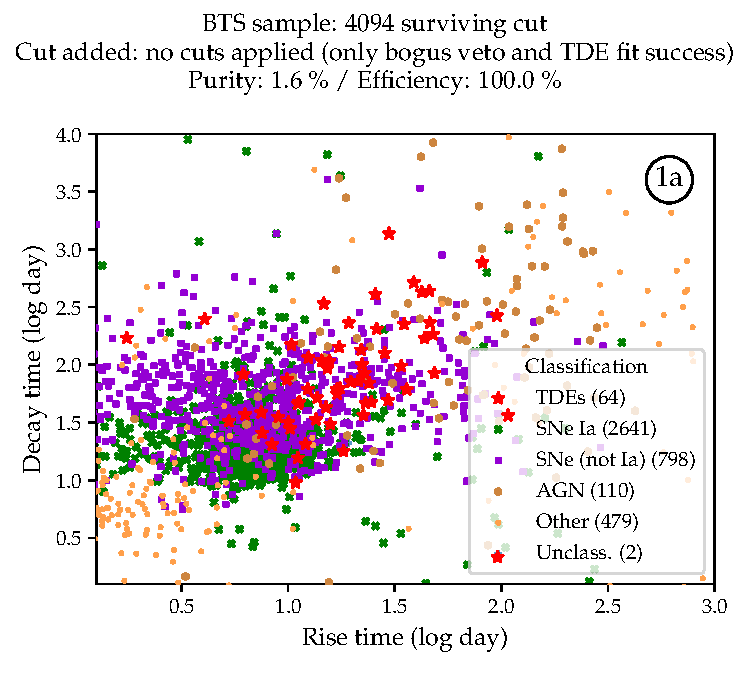
\includegraphics[width=1\textwidth]{nuclear/scatter/tde_rise_decay_['nocut'].pdf}
  \end{subfigure}
  \begin{subfigure}[b]{0.49\textwidth}
    \centering
    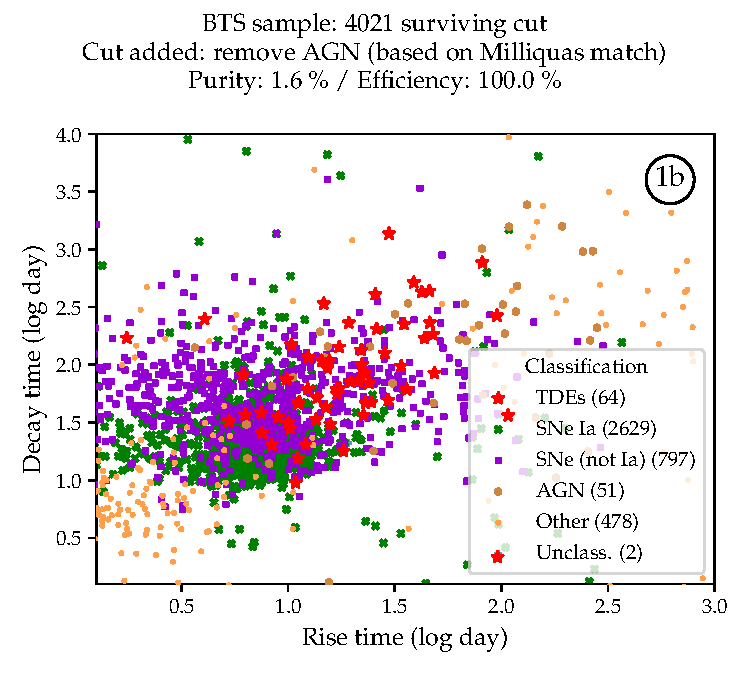
\includegraphics[width=1\textwidth]{nuclear/scatter/tde_rise_decay_['nocut', 'milliquas_noagn'].pdf}
  \end{subfigure}
  \begin{subfigure}[b]{0.49\textwidth}
    \centering
    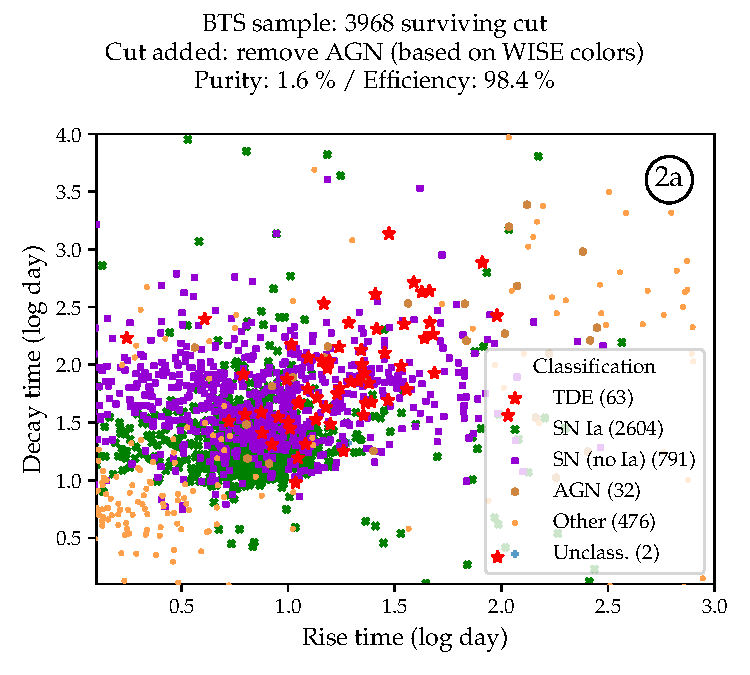
\includegraphics[width=1\textwidth]{nuclear/scatter/tde_rise_decay_['nocut', 'milliquas_noagn', 'wise_noagn'].pdf}
  \end{subfigure}
  \begin{subfigure}[b]{0.49\textwidth}
    \centering
    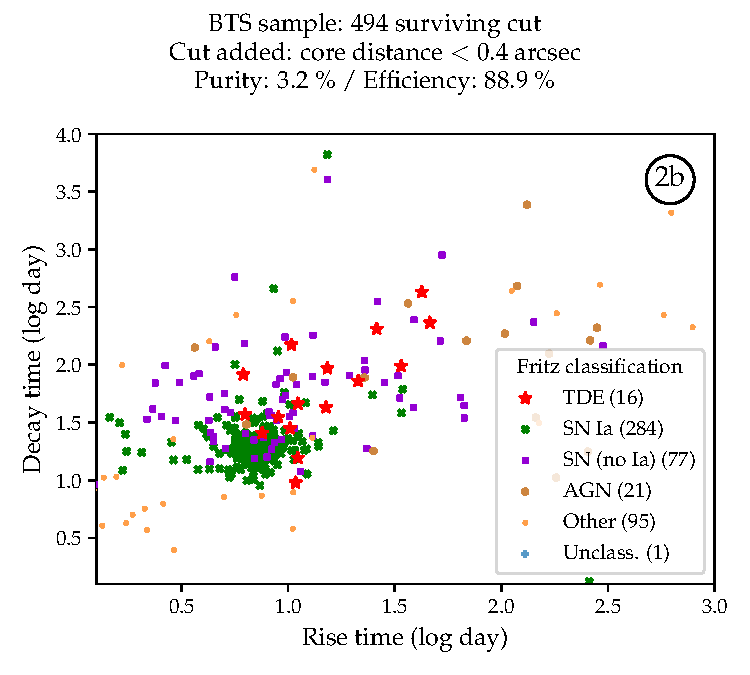
\includegraphics[width=1\textwidth]{nuclear/scatter/tde_rise_decay_['nocut', 'milliquas_noagn', 'wise_noagn', 'coredist'].pdf}
  \end{subfigure}
  \begin{subfigure}[b]{0.49\textwidth}
    \centering
    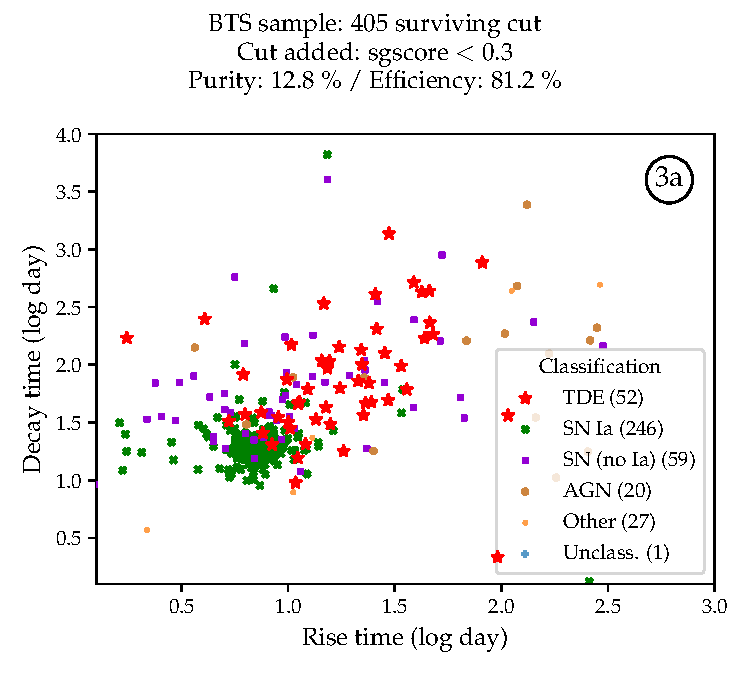
\includegraphics[width=1\textwidth]{nuclear/scatter/tde_rise_decay_['nocut', 'milliquas_noagn', 'wise_noagn', 'coredist', 'sgscore'].pdf}
  \end{subfigure}
  \begin{subfigure}[b]{0.49\textwidth}
    \centering
    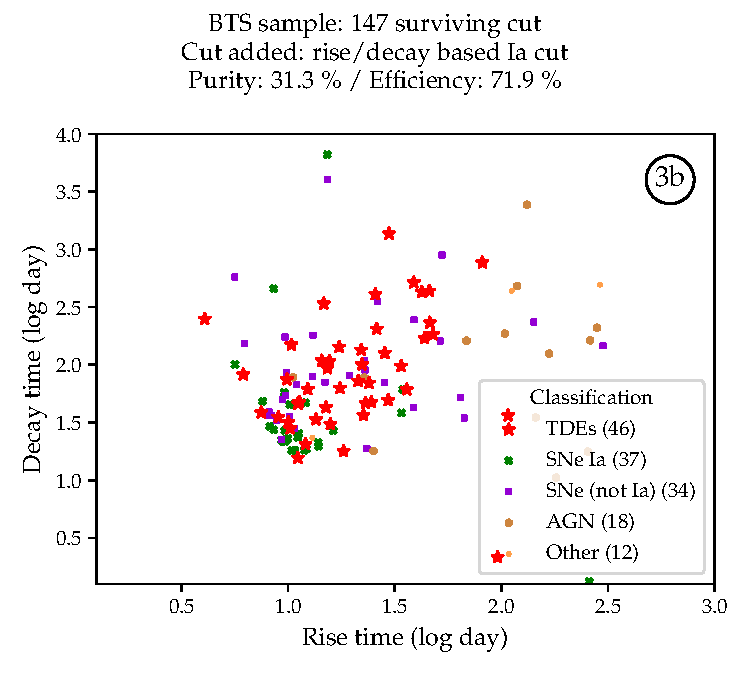
\includegraphics[width=1\textwidth]{nuclear/scatter/tde_rise_decay_['nocut', 'milliquas_noagn', 'wise_noagn', 'coredist', 'sgscore', 'snia'].pdf}
  \end{subfigure}
  \begin{subfigure}[b]{0.49\textwidth}
    \centering
    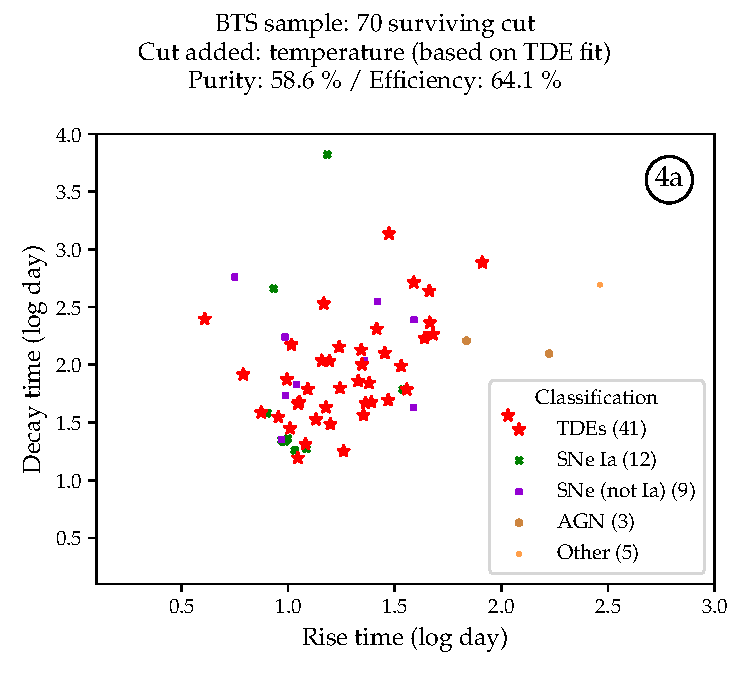
\includegraphics[width=1\textwidth]{nuclear/scatter/tde_rise_decay_['nocut', 'milliquas_noagn', 'wise_noagn', 'coredist', 'sgscore', 'snia', 'temp'].pdf}
  \end{subfigure}
  \begin{subfigure}[b]{0.49\textwidth}
    \centering
    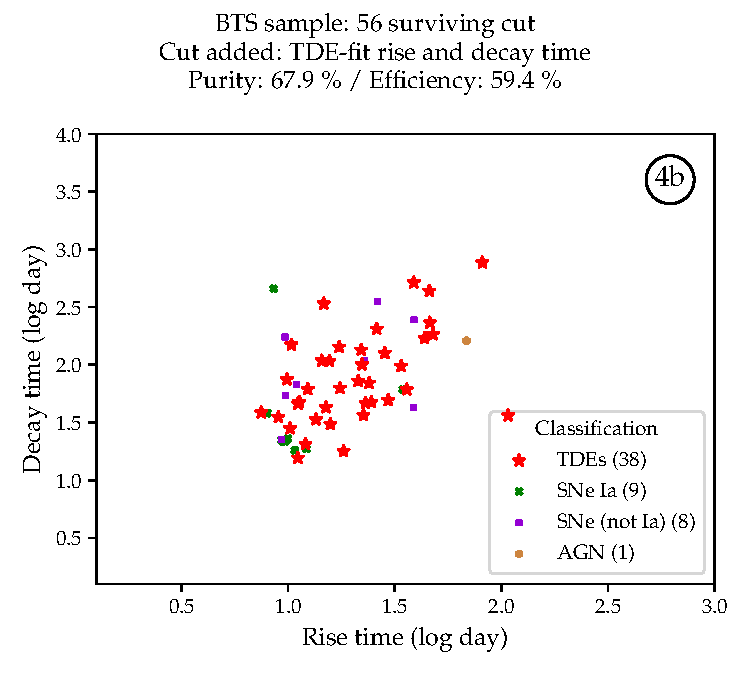
\includegraphics[width=1\textwidth]{nuclear/scatter/tde_rise_decay_['nocut', 'milliquas_noagn', 'wise_noagn', 'coredist', 'sgscore', 'snia', 'temp', 'risedecay'].pdf}
  \end{subfigure}
  \begin{subfigure}[b]{0.49\textwidth}
    \centering
    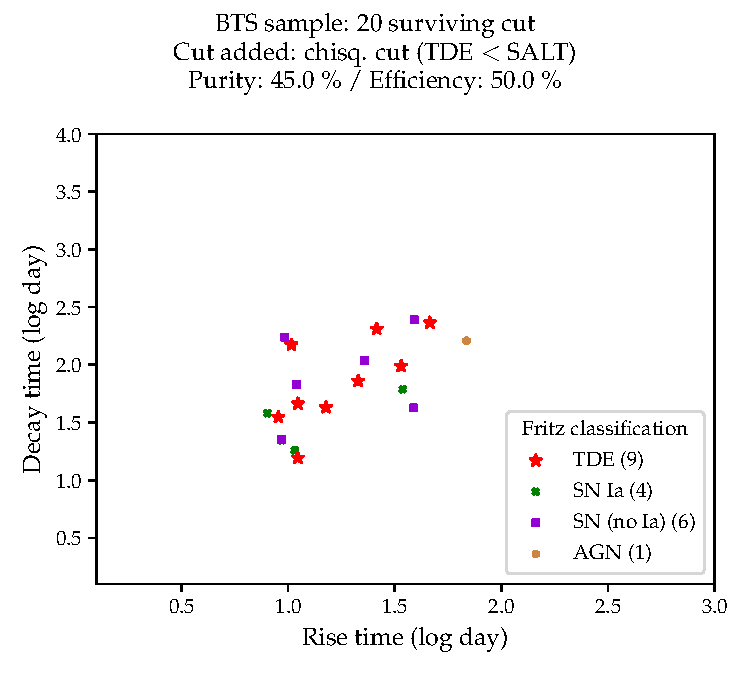
\includegraphics[width=1\textwidth]{nuclear/scatter/tde_rise_decay_['nocut', 'milliquas_noagn', 'wise_noagn', 'coredist', 'sgscore', 'snia', 'temp', 'risedecay', 'chisq'].pdf}
  \end{subfigure}
  \begin{subfigure}[b]{0.49\textwidth}
    \centering
    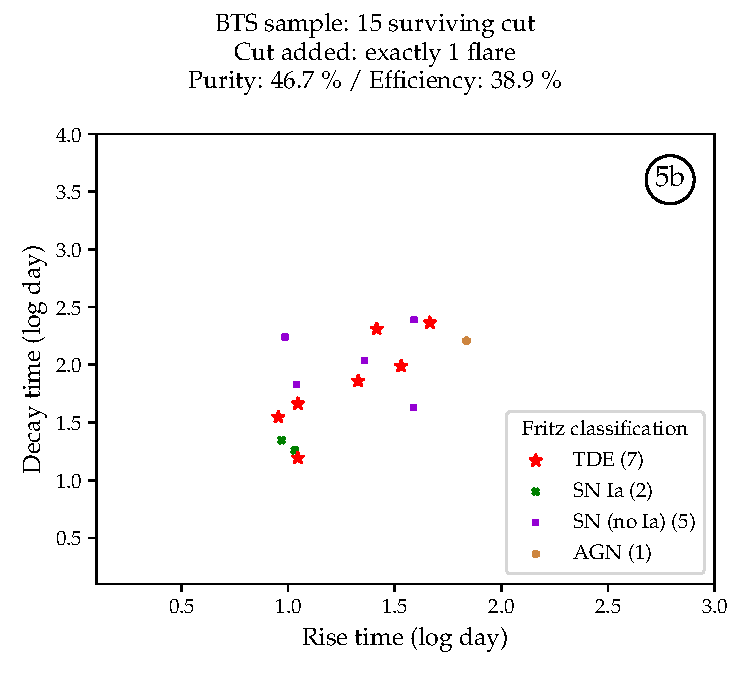
\includegraphics[width=1\textwidth]{nuclear/scatter/tde_rise_decay_['nocut', 'milliquas_noagn', 'wise_noagn', 'coredist', 'sgscore', 'snia', 'temp', 'risedecay', 'chisq', 'bayes'].pdf}
  \end{subfigure}
  \caption[BTS selection]{Visual selection of TDEs among the classified objects of the Bright Transient Survey (augmented with additional TDEs). These are displayed in the rise- and decay-time plane, as derived from the TDE fit (see Section~\ref{tde_model}). From top to bottom and left to right, more and more cuts are added.\newline \newline All classes also used in the training of the classifier are shown. These were TDEs (red stars), SNe Ia (green diagonal crosses), CCSNe (purple squares), AGN (brown hexagons), other types (orange circles), and unclassified objects (blue crosses).\newline \newline \textbf{Top row}: No cuts applied (1a) and the Milliquas-based AGN veto (1b).\newline \newline \textbf{Second row}: AGN cut based on \textit{WISE} colors (2a) and cut based on the core distance (2b).\newline \newline \textbf{Third row}: The \texttt{sgscore} is required to lie below 0.3 (3a) and SNe Ia are removed by a diagonal cut in the rise-/decay time plane (3b)\newline \newline \textbf{Fourth row}: The temperature and temperature evolution were restricted (4a), as were the rise and decay times (4b). \newline \newline \textbf{Bottom row}: Finally, it was required that the TDE model was a better fit than the SALT2 model by requiring the reduced $\chi^2$ of the TDE fit to be smaller than the SALT2 fit's $\chi^2$ (5a), and that the transient light curve had exactly 1 flare (5b).}
  \labfig{bts_scatter}
\end{figure}

After establishing and verifying the visual cuts, everything is ready to use the visual cuts on the model predictions and investigate its performance further.

\section{A Photometric TDE sample}
As we know obtained a trained classifier and a set of visual cuts optimized for isolating TDE candidates, the next step is to classify the nuclear sample with the trained model, and subject it to the visual cuts.

\subsection{Running the Classifier}
The full classification of the nuclear sample is shown in Fig.~\ref{fig:classification_maghist_nocut}. Here, the plots on top only show \textbf{non-AGN hosts}, while the bottom plots show likely \textbf{AGN hosts}. This differentiation was again achieved by crossmatching the Milliquas catalog and using the \textit{WISE} colors (see Section~\ref{agn_rejection}). The plots on the left show community classifications drawn from Fritz, the GROWTH Marshal and the TNS, while the right side plots display the \texttt{XGBoost} classifications.

\begin{figure}[H]
  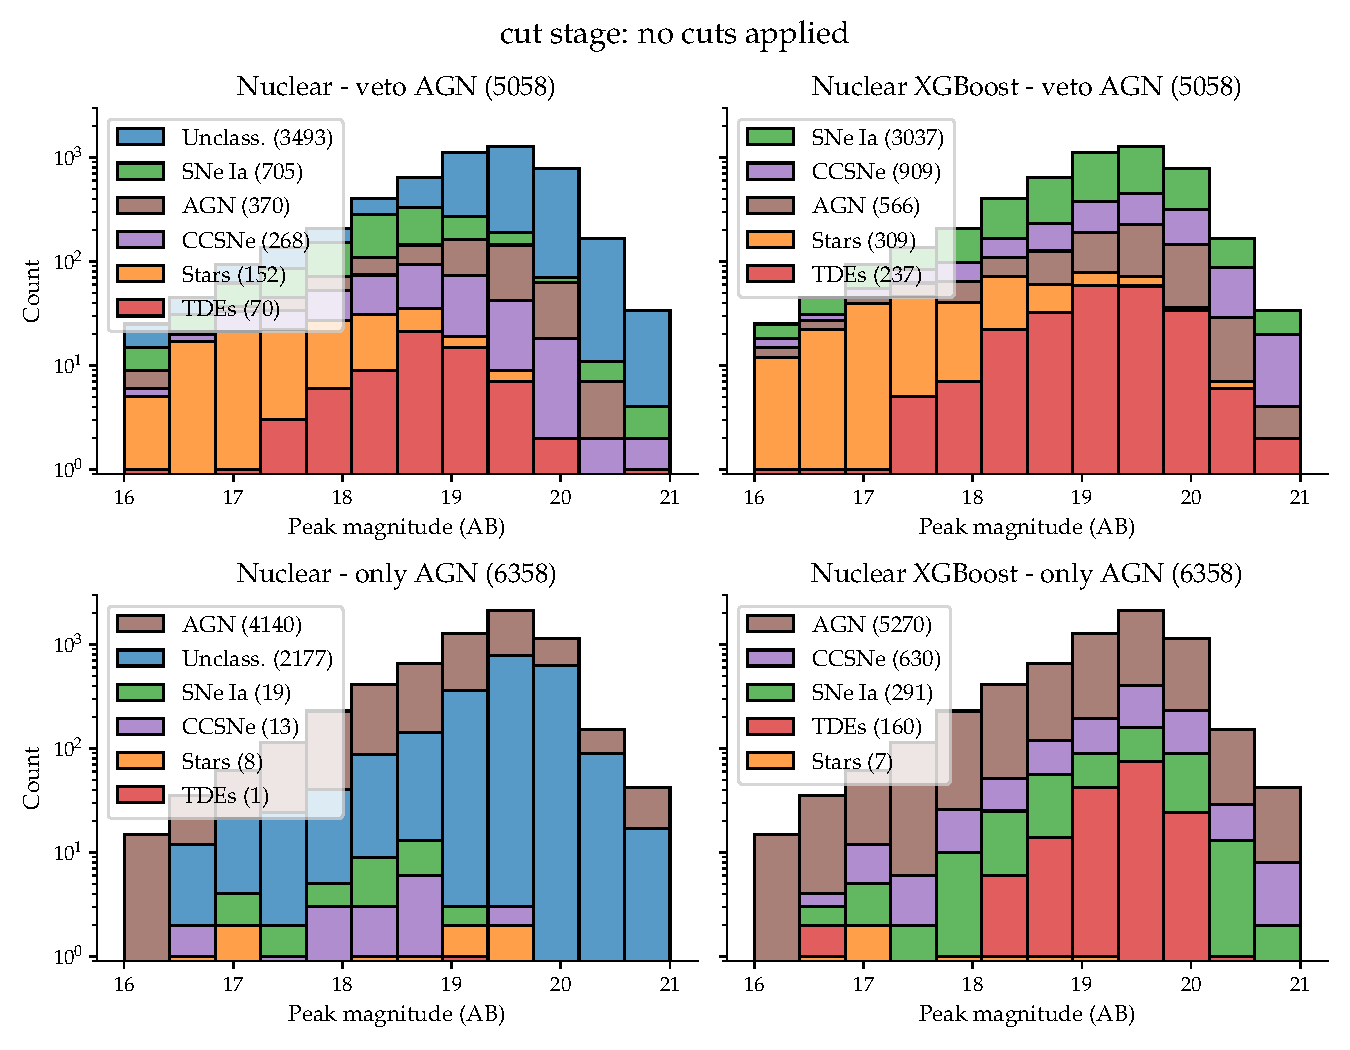
\includegraphics[width=1\textwidth]{nuclear/maghist/maghist_['nocut']_comb.pdf}
  \caption[Classification without cuts]{Classifications of the \texttt{XGBoost} model. This figure shows the nuclear sample, binned in magnitude steps of $0.5$. There are no cuts applied. The classifications on the left side come from the community, i.e.~Fritz, the GROWTH Marshal or TNS. The plots on the right side show the \texttt{XGBoost} classifications. The top row shows non-AGN hosts, while the bottom row shows likely AGN hosts.}
  \labfig{classification_maghist_nocut}
\end{figure}

Looking at the AGN part of the nuclear sample (bottom right plot), one can notice that reassuringly the majority (\SI{83}{\percent}) was indeed classified as AGN by the decision tree. As it is much more likely to contain bona-fide transients, we will now focus on the non-AGN part of the nuclear sample (top right plot). At this stage, without further cuts on the sample, \texttt{XGBoost} classified 3037 objects as SN Ia, 909 as CCSN, 566as AGN, 309 as stars, and 237 as TDE.

\begin{figure}[htpb]
  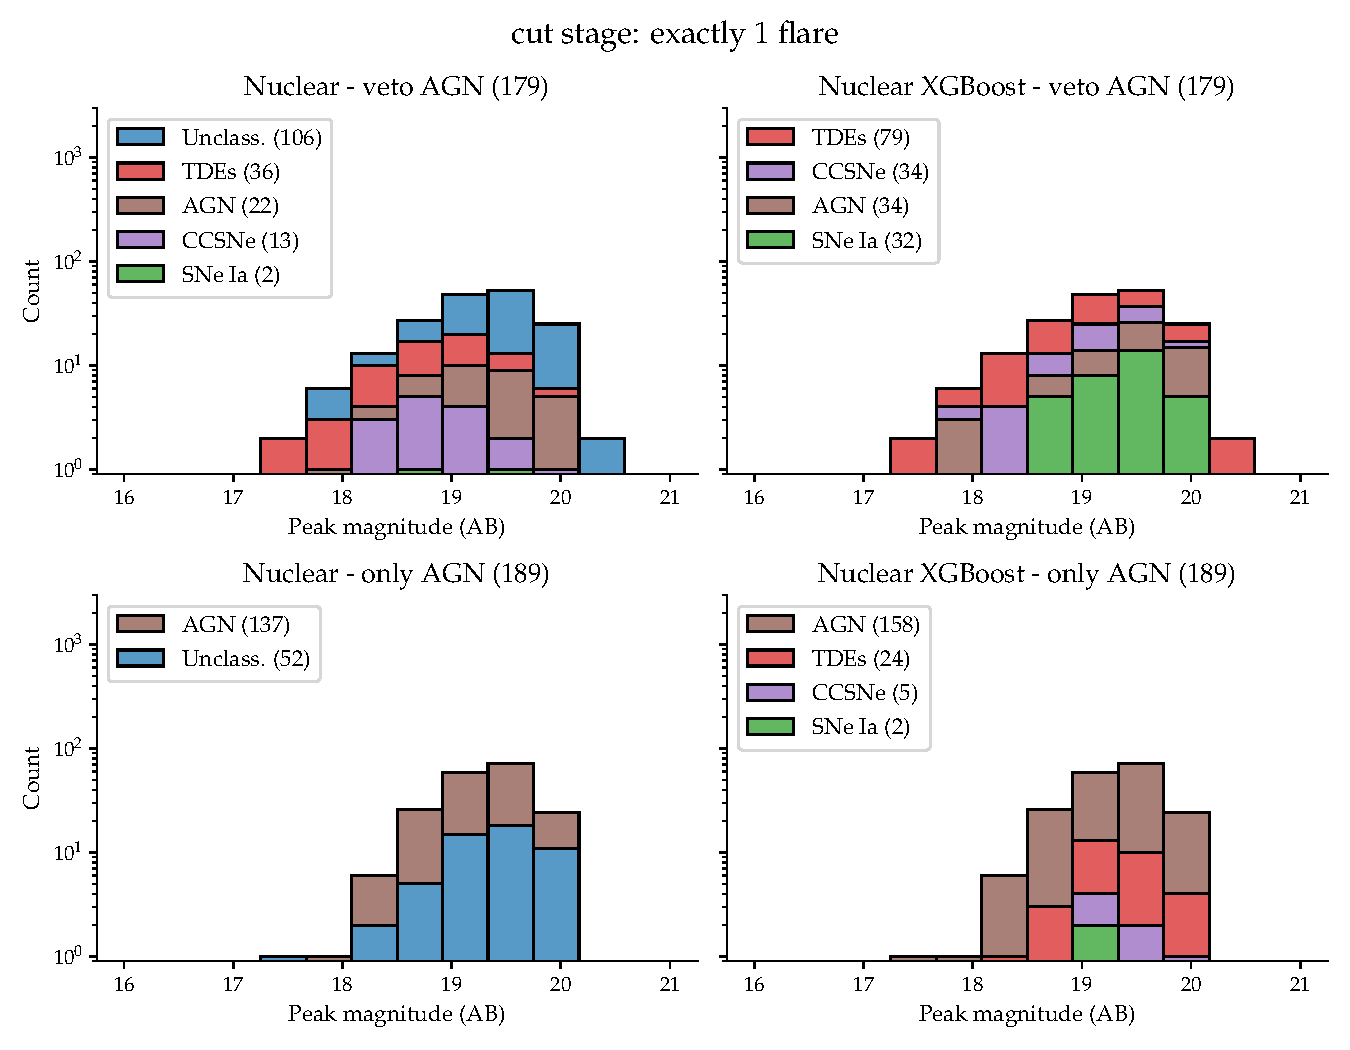
\includegraphics[width=1\textwidth]{nuclear/maghist/maghist_['nocut', 'coredist', 'sgscore', 'snia', 'temp', 'risedecay', 'chisq', 'bayes']_comb.pdf}
  \caption[Classification with all visual cuts]{Classifications of the \texttt{XGBoost} model, this time with all the visual cuts applied. Left side: community classifications, i.e. from~Fritz, the GROWTH Marshal or TNS; right side: \texttt{XGBoost} classifications. Top row: non-AGN hosts; bottom row: likely AGN hosts.}
  \labfig{classification_maghist_cut}
\end{figure}

To obtain a purer (but of course less complete) TDE sample, the visual cuts established in Section~\ref{visual_cuts} were applied. The classification of nuclear sample after application of these cuts can be seen in Fig.~\ref{fig:classification_maghist_cut}. The full list of all 79 transients from non-AGN hosts classified as TDE, including new and already known ones can be found in the Appendix, see Table~\ref{tab:tde_candidates}. In total, \textbf{26 TDE candidates could be added} to the already known and established TDEs.

Unfortunately, visual inspection of the 24 events within AGN hosts that were identified as TDE ruled out all but one (\textit{ZTF18acryjql}) transient. This was almost always possible based on light curve features alone, highlighting \textbf{potentially lacking performance of the classifier}.

\subsection{Inspection of Objects Classified as TDE}\label{all_tde_inspection}
One pitfall in evaluating the classifier performance is the fact that \SI{70}{\percent} of all TDEs were already seen by the classifier in the training stage --- this was neccessitated by the fact that there were not many to begin with. Therefore, a visual inspection of all objects classified as TDE that were not already known as TDEs during the training stage was performed.
\todo{work in progress}

\subsection{Conclusions}
The performance of the classifier yielded somewhat mixed results. There was a number of problems identified that need to be addressed when improving the classification quality:

\begin{description}
  \item[Data quality] In some cases, inspection of transients classified as TDE showed a sparsely sampled light curve, e.g.~\textit{ZTF21aanubdr}~\sidenote{\url{https://ztfnuclear.simeonreusch.com/transient/ZTF21aanubdr}}. A human would recognize that the sparse sampling allows only little conclusions to be drawn, while the decision tree had no adequate way of reacting to that fact. It would be beneficial to somehow infer from the data quality the range of conclusions that could possibly be drawn for a specific object.
  \item[Misclassifications] There were examples where visual inspection allowed for easy and straightforward classification --- especially in the case of stochastic AGN variability --- but the classifier struggled to identify the AGN-nature of the transient. This highlights that there might still be room for improvement, i.e.~further features that humans easily grasp and which could be exploited for automatic classification. The `exactly 1 coincident flare' feature was apparently not sufficient for this task, and neither was the the high $\chi^2$ of the TDE and SALT2 fits.
  \item[Effectiveness of Augmentation] The TDE classification performance of the classifier when applied to the nuclear sample was investigated (see Section~\ref{all_tde_inspection}). The results were worse than the confusion matrices of the test sample (see Section~\ref{confusion_matrices}) suggested: \xx of 201 objects classified as TDE and not seen by the classifier during training are most likely something else, a much higher false-positive rate than the test sample suggested (\xx). This means that the augmentation by creating redshifted and noisified copies was not able to fully capture the transition from the BTS sample to the nuclear sample.
\end{description}

\section{Selection by Dust Echo}\label{dustecho_sel}
A final avenue of obtaining interesting, hitherto missed nuclear transients was a selection based on their infrared dust echo. For this, all transients with a \texttt{T2DustEchoEval} result (see Section~\ref{irdata}) suggesting the existence of an infrared flare occuring simultaneous to or after the optical peak were visually inspected.

\subsection{Inspection Tool}
To aid in the visual inspection of light curves, the author created a web-based frontend to interactively view the light curves of the nuclear sample, especially the ones showing an infrared flare qualifying for a dust echo. This tool, still accessible under \url{https://ztfnuclear.simeonreusch.com}, was written in Python. It is based on the \texttt{Flask}\sidenote{\url{flask.palletsprojects.com}} web framework, and operated behind an \texttt{nginx} web server also serving a reverse proxy on a virtual private server.

Fig.~\ref{fig:ztfnuclear_frontend} shows a screenshot of the frontend. This was designed to display the transient light curve, results from the crossmatching, a redshift if one were found, as well as links to object pages on the GROWTH Marshal, Fritz and TNS. Lastly, it has the possibility to leave comments (this is why a login system was created) and to rate the transient as `interesting', `maybe interesting', and `boring'.

\begin{figure}[htpb]
  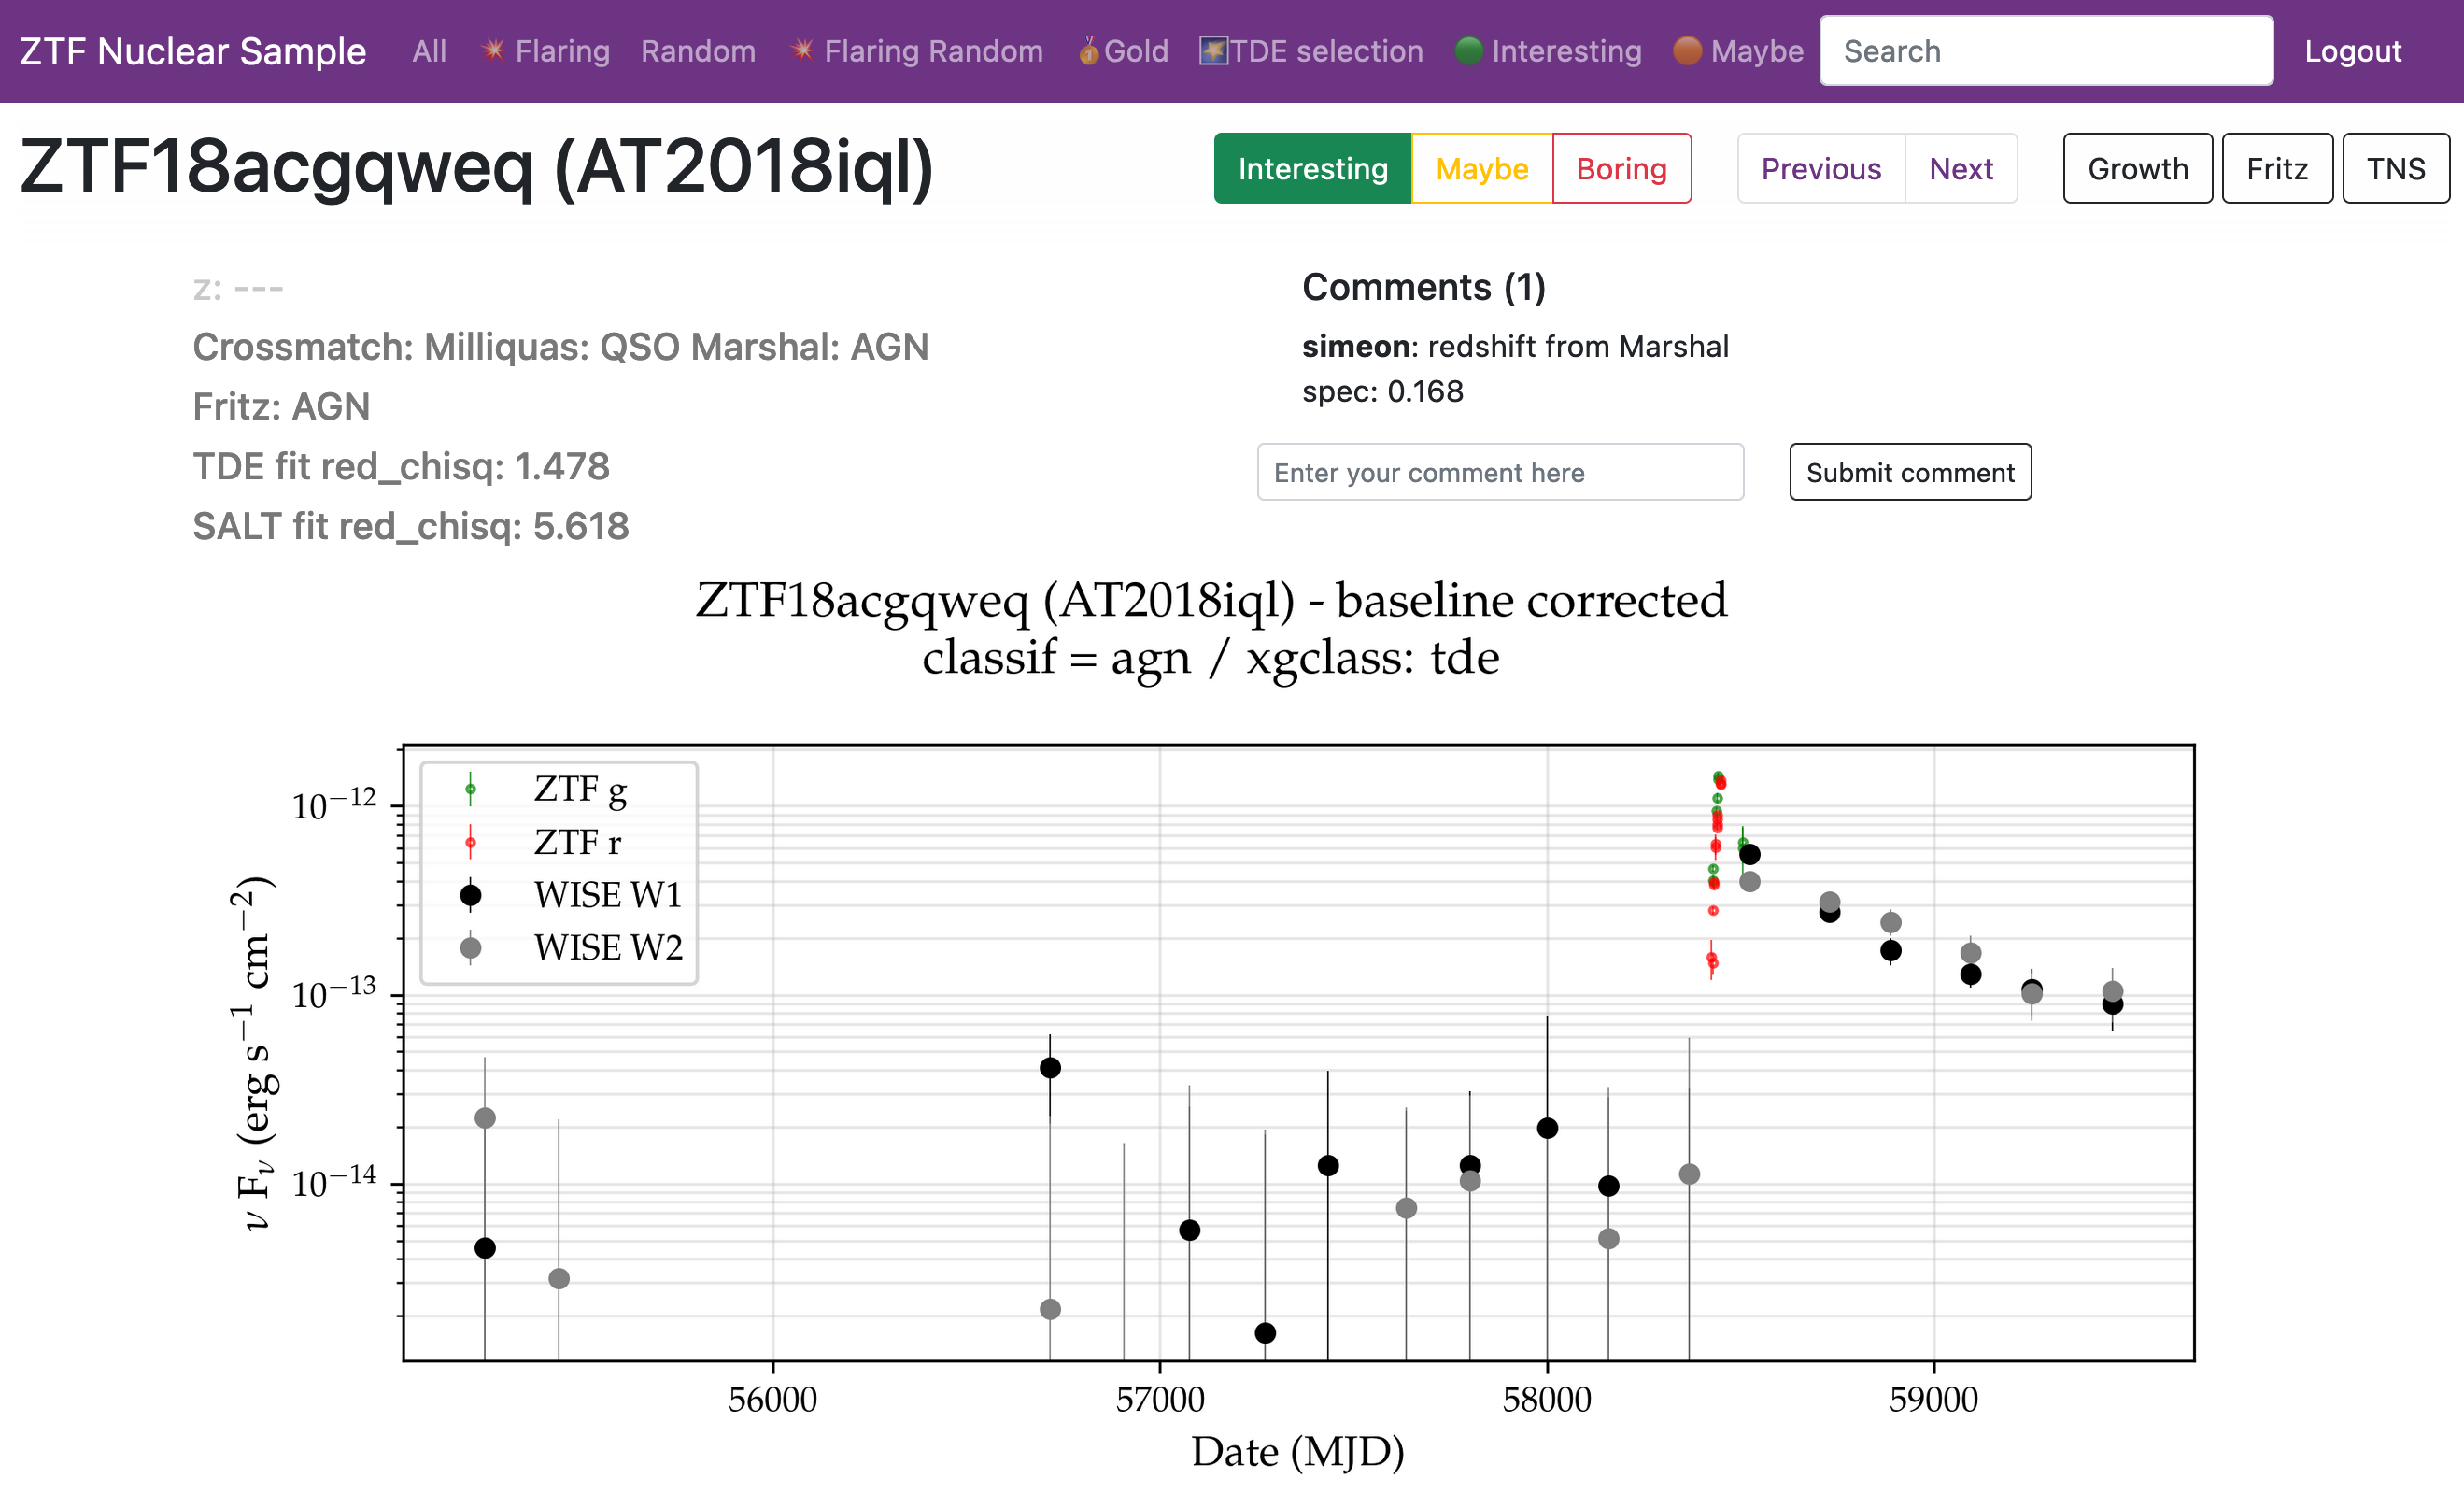
\includegraphics[width=1\textwidth]{nuclear/ztfnuclear_frontend.png}
  \caption[Frontend for the nuclear sample]{The frontend for inspecting and reviewing the nuclear sample. It shows an exemplary page for \textit{ZTF18acgqweq}, including a light curve, a comment and a rating as `Interesting'. The fit results of the TDE and the SALT2 fit are displayed as well, plus potential redshift matches (none in this case).}
  \labfig{ztfnuclear_frontend}
\end{figure}

\subsection{Creating a Gold Sample}
To create a sample of dust echo transients that look promising, multiple users review all transients with a \texttt{T2DustEchoEval} score of 1, designed to select likely real infrared flares compatible with a dust echo. A dust echo evaluation score of 1 selects infrared flares that have reliable baseline in both bands before the flare, and the flare is evolving reasonably fast (rise time $<1000$ days, fade time $<5000$ days).

The review was performed using the web frontend, and each user rated the transients as either `interesting', `maybe interesting' or `boring'. The final selection comprises transients that were rated as `interesting' by at least two users.

An overview table of the 37 transients that met this criterion can be seen in the Appendix in Table~\ref{tab:dustecho_selection}.

\subsection{New TDE and Accretion Flare Candidates}
Among this final selection were 15 TDE or accretion flare candidates that showed a strong dust echo, and which were not published so far. These comprise:

\textit{\href{https://ztfnuclear.simeonreusch.com/transient/ZTF18abnwufa}{ZTF18abnwufa}}, \textit{\href{https://ztfnuclear.simeonreusch.com/transient/ZTF18abtnfnq}{ZTF18abtnfnq}}, \textit{\href{https://ztfnuclear.simeonreusch.com/transient/ZTF19aamsgro}{AT2019cyq}}, \textit{\href{https://ztfnuclear.simeonreusch.com/transient/ZTF20aaidhtp}{ZTF20aaidhtp}}, \textit{\href{https://ztfnuclear.simeonreusch.com/transient/ZTF20aaostow}{ZTF20aaostow}}, \textit{\href{https://ztfnuclear.simeonreusch.com/transient/ZTF20aaoxtxi}{AT2020ima}}, \textit{\href{https://ztfnuclear.simeonreusch.com/transient/ZTF20aauvhab}{AT2020hip}}, \textit{\href{https://ztfnuclear.simeonreusch.com/transient/ZTF20abgxlut}{AT2020oio}}, \textit{\href{https://ztfnuclear.simeonreusch.com/transient/ZTF20abhrmri}{AT2020nnc}}, \textit{\href{https://ztfnuclear.simeonreusch.com/transient/ZTF20ablvwmh}{AT2020xtj}}, \textit{\href{https://ztfnuclear.simeonreusch.com/transient/ZTF20abxtsgg}{ZTF20abxtsgg}}, \textit{\href{https://ztfnuclear.simeonreusch.com/transient/ZTF20acyxxfo}{AT2020aetz}} and \textit{\href{https://ztfnuclear.simeonreusch.com/transient/ZTF21aaekxxf}{AT2021esn}}.

Two exemplary light curves are shown in Fig.\ref{fig:two_dustecho_examples}, one candidate TDE (\textit{ZTF18abtnfnq}), and one candidate accretion flare similar to \textit{AT2019fdr}: \textit{AT2020oio}.

\begin{figure}[htbp]
  \centering
  \begin{subfigure}[b]{1\textwidth}
    \centering
    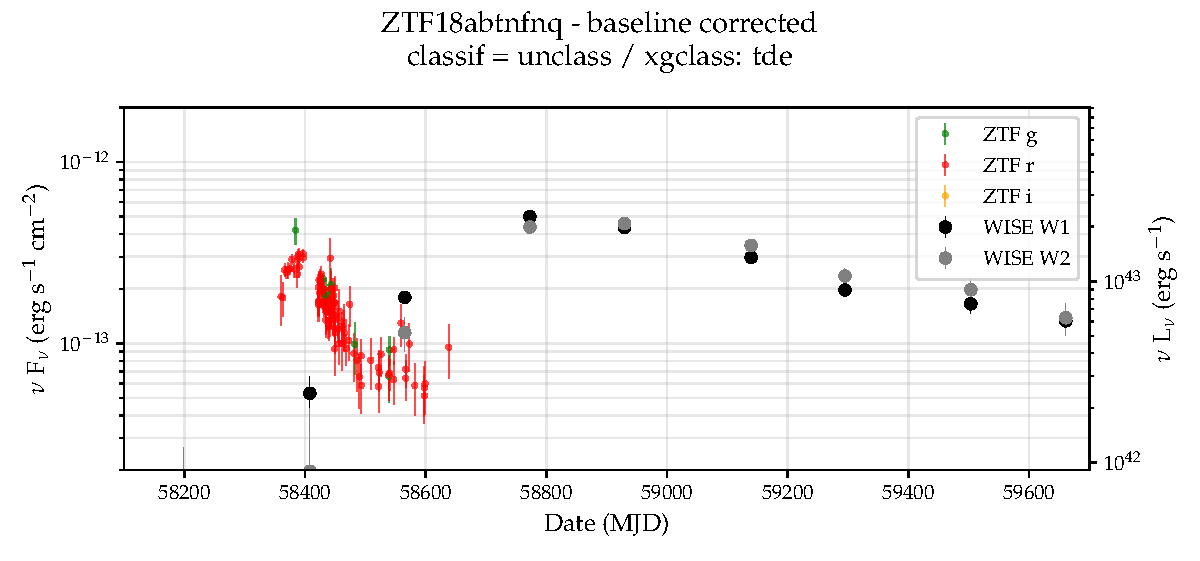
\includegraphics[width=1\textwidth]{nuclear/ZTF18abtnfnq.pdf}
  \end{subfigure}
  \begin{subfigure}[b]{1\textwidth}
    \centering
    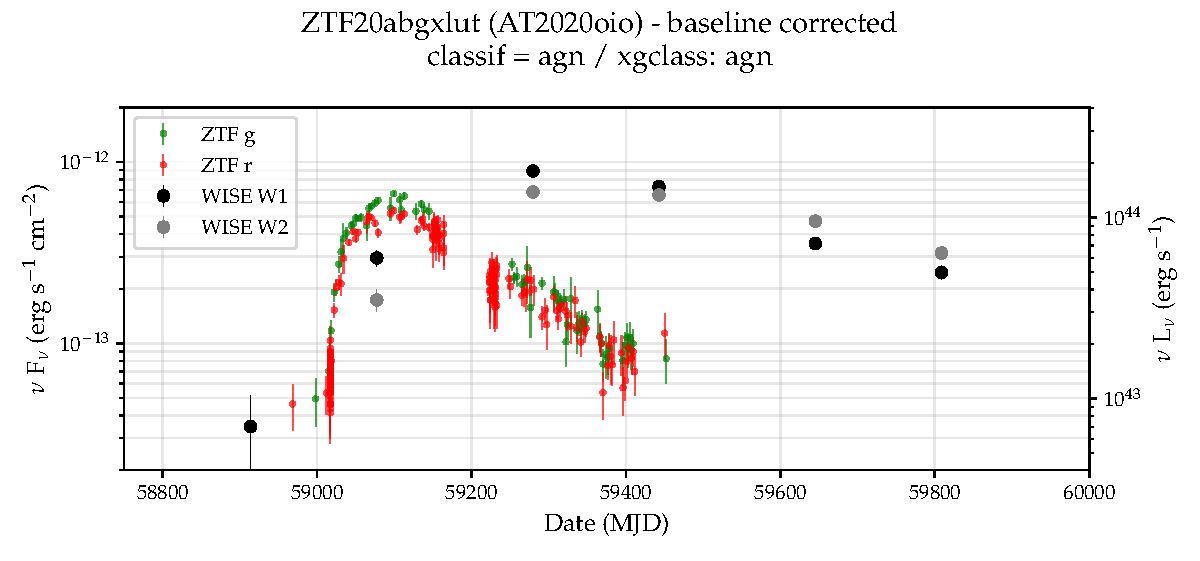
\includegraphics[width=1\textwidth]{nuclear/ZTF20abgxlut.pdf}
  \end{subfigure}
  \caption[Two exemplary light curves from the dust echo selection]{Two exemplary light curves from the dust echo section. Top: TDE candidate \textit{ZTF18abtnfnq}. Bottom: Accretion flare candidate \textit{ZTF18abtnfnq}. Both have spectacular dust echoes. On the top, the delay between optical and infrared peak is roughly 400 days, while on the bottom it is about 180 days.}
  \labfig{two_dustecho_examples}
\end{figure}

\section{Conclusion}

% Prelim. study of the sample shows that there are at least xx more likely TDEs and dust echo, ongoing work on multiple levels

% a) slightly more involved theoretical model study
% b) realtime pipeline conversion maybe possible
% c) realtime application of the wise / lsst dust detection capabilities?

% is the accretion stuff vs. agn just a continuum?

